\documentclass[review,authoryear]{elsarticle}

% Encoding and fonts
\usepackage[T1]{fontenc}
\usepackage[utf8]{inputenc}
\usepackage{microtype}

% Math
\usepackage{amsmath,amssymb}

% Tables
\usepackage{longtable,booktabs,array}
\usepackage{calc}
\usepackage{etoolbox}
\makeatletter
\patchcmd\longtable{\par}{\if@noskipsec\fi\par}{}{}
\makeatother
\usepackage{footnote}
\makesavenoteenv{longtable}

% Graphics
\usepackage{graphicx}
\usepackage{float}
\usepackage{placeins}
\graphicspath{{../figures/}{figures/}{./}}
\def\fps@figure{htbp}

% Links
\usepackage[hidelinks]{hyperref}
\usepackage{url}
\urlstyle{same}

% Line numbers (required for review)
\usepackage{lineno}

% Lists
\providecommand{\tightlist}{%
  \setlength{\itemsep}{0pt}\setlength{\parskip}{0pt}}

\setlength{\emergencystretch}{3em}

\journal{Transportation Research Interdisciplinary Perspectives}

%% ============================================================
\begin{document}

\begin{frontmatter}

\title{Demand Synchronization Dominates Urban Traffic Congestion: Evidence from 264 Million Observations across Three Indonesian Cities}

\author[undip]{Firman Hadi\corref{cor1}}
\ead{firmanhadi21@lecturer.undip.ac.id}
\author[undip]{Yasser Wahyuddin}
\author[undip]{L.M. Sabri}
\author[nca]{Agung Indrajit}

\affiliation[undip]{organization={Department of Geodetic Engineering, Universitas Diponegoro},
  city={Semarang}, country={Indonesia}}
\affiliation[nca]{organization={Deputy for Green and Digital Transformation, Nusantara Capital Authority},
  country={Indonesia}}

\cortext[cor1]{Corresponding author.}

\begin{abstract}
Urban traffic congestion is widely attributed to infrastructure bottlenecks---insufficient road capacity, poor network connectivity, or land-use mismatches---yet the relative contribution of \emph{when} versus \emph{where} people travel remains poorly quantified in rapidly urbanizing cities with motorcycle-dominated traffic. This study analyzes 264 million traffic observations collected at 15-minute intervals across Jakarta, Bandung, and Semarang over 11 months to empirically decompose congestion into its temporal and spatial components. Using multilevel mixed-effects models on absolute speed, we find that demand synchronization---millions of commuters traveling simultaneously---is the primary congestion mechanism: time-of-day explains 57--67\% of within-segment speed fluctuations, while network centrality adds less than 1\% beyond road type. A positive-control test confirms that the same analytical pipeline successfully detects spatial structure in road design ($R^2 = 0.60$--$0.71$ for free-flow speed) but not in congestion ($R^2 < 0.003$), ruling out methodological artefacts. Cross-metric validation using absolute speed, jam factor, and speed reduction confirms these patterns are not normalization artefacts. Evening peak congestion exceeds daily averages by approximately 40\% across all three cities despite a 20$\times$ population range, consistent with a demand-driven rather than supply-constrained mechanism. These findings imply that demand management interventions (congestion pricing, flexible work schedules, public transit) may yield greater returns than capacity expansion alone in rapidly urbanizing contexts.
\end{abstract}

\begin{keyword}
Urban traffic congestion \sep Spatiotemporal analysis \sep Demand synchronization \sep Network centrality \sep Multilevel model \sep Indonesian cities \sep OpenStreetMap
\end{keyword}

\end{frontmatter}

%% Graphical abstract: submit paper/graphical-abstract.png as a separate file

\linenumbers

\section{Introduction}

Urban traffic congestion poses a major challenge for rapidly growing cities in developing countries, characterized by high variability, peak periods, and reliance on informal transportation systems \citep{Gakenheimer1999,Pojani2015}. The economic impact is substantial: in Southeast Asia, congestion costs are estimated at 2--5\% of GDP each year \citep{ADB2019}, while welfare losses from transport-related air pollution amount to 4.8\% of GDP in East Asia and 3.5\% in South Asia \citep{WorldBank2022}. The Western Pacific and Southeast Asia regions face the highest levels of traffic-related air pollution, reflecting the rapid urbanization in these developing nations \citep{WHO2021}. Accelerating urbanization and population growth have increased the demand for urban infrastructure, leading to persistent congestion that traditional planning methods often cannot fix \citep{Cervero2013}. Cities across Southeast Asia, South Asia, and Sub-Saharan Africa face similar problems: vehicle numbers grow faster than road capacity, motorcycle use is high, public transit systems are inadequate, and data for evidence-based planning is limited \citep{Pojani2015,Kutzbach2009}. The advent of big data analytics has begun to transform our understanding of these urban dynamics \citep{Batty2013}, but a lack of data often limits traffic improvement efforts to places where congestion is easiest to measure.

Indonesia vividly illustrates these challenges. Jakarta has long struggled with severe traffic jams, and recent studies show that Bandung, Semarang, Surabaya, and Yogyakarta now face similar congestion issues. The World Bank reports that Jakarta is among the most traffic-congested cities worldwide, with commuters spending an average of 62 hours annually in traffic and economic losses projected to reach US\$6.5 billion by 2020. Peak-hour vehicle speeds are only about 10 km/h \citep{WorldBank2021}. Castrol notes that Jakarta drivers experience roughly 33,240 stop-starts each year, with 27\% of travel time spent stationary \citep{Castrol2015}. Bandung, Indonesia's second-largest city, ranks second among 38 Indonesian cities in a World Bank analysis, with peak-hour speeds of only 17 km/h \citep{WorldBank2019}. The Asian Development Bank identified Bandung as Indonesia's most congested city and 14th in Asia \citep{ADB2019}. A notable feature of Indonesian urban traffic is the very high motorcycle share; in Bandung, motorcycles accounted for 72.2\% of vehicles in 2013 \citep{BPSBandung2015}, creating traffic flows that differ significantly from those in car-dominated systems in developed nations. Earlier Indonesian traffic research mainly relied on surveys: \citet{Susilo2007} examined motorization and public transport trends in Jakarta, while \citet{Joewono2008} studied paratransit user satisfaction. More recent studies focus on demand management measures such as car-free days and odd-even plate policies in Bandung \citep{Farda2020}. However, these often provide only snapshot views rather than continuous traffic dynamics. Although Indonesia has prioritized mass transit development in six metropolitan areas through projects such as the Indonesia Mass Transit Project \citep{WorldBank2022}, comprehensive empirical analysis of congestion patterns using high-resolution data remains limited, hindering evidence-based planning of interventions.


Recent international traffic research increasingly uses multi-source data and advanced analytical frameworks to understand urban congestion patterns. In China's largest cities, real-time traffic data from online maps has been used to identify frequently congested road segments, showing that 1.8--9.87\% of urban road networks face chronic congestion and that congestion severity correlates with city size \citep{Cui2024}. Similar methods in Shanghai during and after the COVID-19 pandemic have shown how disruptions changed spatiotemporal congestion trends \citep{Xu2022}. In South Asia, Dhaka has been a case study for analyzing the effects of urbanization on traffic, with researchers combining satellite-based traffic and pollution data with socioeconomic information. In Tanzania, Dar es Salaam has been examined using European Space Agency Sentinel-5P satellite data to associate traffic congestion with air pollution exposure \citep{Dasgupta2021}. These studies show that remote sensing and crowdsourced data can support detailed analyses in cities without traditional traffic-monitoring systems. Combining multi-source data with high-performance computing allows for measuring key spatiotemporal patterns in human mobility and congestion \citep{Cai2024}, although machine learning methods still face challenges in effectively merging temporal features with network topology for congestion prediction \citep{Song2019,Ermagun2018}.

The availability of probe vehicle data and APIs has advanced traffic analysis by enabling high-resolution, broad coverage \citep{Leduc2008,Jenelius2015}. Floating car data (FCD) from GPS vehicles offers a cost-effective alternative to fixed sensors for large-scale traffic assessment \citep{Zhang2025}. Studies show that leveraging FCD and a Spatial-Temporal Autoformer (STAF) can significantly improve data validity (90.2\%) and road network coverage (85.7\%) compared to traditional data collection \citep{Ma2024}. Commercial APIs from HERE, TomTom, and Google are vital for urban traffic research. HERE's data combines information from various sources across 70+ countries and 13 million km of roads \citep{HERE2024}. The jam factor, which ranges from 0 (free) to 10 (standstill), supports cross-network comparisons and has been used to analyze the spatiotemporal spread of congestion in European cities \citep{Rempe2016,Saberi2020}. Crowdsourced data research has expanded from Western cities to developing regions, such as Al Ain (UAE), building on methods from Windsor, Toronto, and New York \citep{Alkaabi2024}. However, most studies analyze a single city using snapshot data, rely on descriptive statistics, and focus more on visualization than on hypothesis testing. No studies have systematically tested whether spatial factors predict congestion while controlling for time, or compared congestion across multiple cities with hundreds of millions of observations. Research is also limited in Southeast Asia and Indonesia, where motorcycles create unique traffic dynamics.

Alongside advancements in data, the OSMnx framework \citep{Boeing2017} has improved capabilities for large-scale street network analysis, allowing systematic exploration of urban infrastructure topology and the calculation of transportation-related metrics, including intersection density, circuity, average node degree, and centrality measures \citep{Boeing2025}. Betweenness centrality---measuring the proportion of shortest paths passing through each node or edge---has been hypothesized to relate to traffic volumes, with studies finding significant links in some urban contexts \citep{Gao2013,Porta2006}. However, empirical evidence varies: research in Portland showed that grid-like networks distribute importance more evenly (15\% of paths through the most central node) than constrained networks (43\%), suggesting that topology--congestion relationships depend on network structure \citep{Boeing2018,Kirkley2018}. The traffic bottleneck theory further posits that reductions in roadway capacity focus congestion at specific points \citep{Daganzo2007,Arnott1993}, but empirical evidence linking static capacity features directly to city-wide congestion remains limited. Grounded in Tobler's first law of geography \citep{Tobler1970}---that near things are more related than distant things---spatial autocorrelation methods offer powerful tools for identifying traffic clusters: Global Moran's I evaluates overall spatial clustering \citep{Moran1950}, while Local Indicators of Spatial Association (LISA) identify specific hotspot and coldspot locations \citep{Anselin1995}. Getis-Ord Gi* statistics complement LISA by detecting statistically significant spatial concentrations \citep{Getis1992,Ord1995}. These techniques have been widely used in traffic crash analysis---\citet{Gedamu2024} compared crash severity clustering in Addis Ababa and Berlin using Moran's I---but applications to real-time congestion data are still less common, especially in developing country contexts.

Despite the increasing availability of probe vehicle data and commercial traffic APIs, systematic spatiotemporal analysis of urban congestion in Indonesia using high-resolution data remains limited. Past Indonesian studies relied mainly on surveys or short-term observations, lacking continuous long-term monitoring. The combination of network topology metrics with traffic flow data is still underexplored, and whether physical capacity constraints can predict congestion patterns has not been thoroughly tested in these contexts. The three cities studied here --Jakarta, Bandung, and Semarang -- represent different types of Indonesian urban environments. Jakarta, a megacity of 10.5 million residents (metro: 34 million), consistently ranks among the world's most congested cities \citep{TomTom2023} and has high motorcycle volumes exceeding 60\%. Bandung (2.5 million) is Java's second-largest city, located in a highland basin with limited network development. Semarang (1.8 million), serving as Central Java's logistics hub, stretches across coastal lowlands and southern hills, forming distinct traffic zones.

This study addresses gaps with four methods: analyzing 11 months of traffic data totaling over 264 million observations; using geostatistical techniques like Moran's I, LISA, and Getis-Ord Gi* to identify clusters; applying OSMnx network analysis to link topology and congestion; and testing if capacity constraints, including a new graph-based capacity drop detection, predict congestion. The research offers five key contributions: (1) empirical evidence that urban congestion operates as a demand synchronization phenomenon, with time-of-day explaining 57--67\% of speed variation while network topology adds less than 1\% beyond road type; (2) a positive-control methodology demonstrating that the same analytical pipeline detects spatial structure in road design but not in congestion, ruling out methodological artefacts; (3) cross-metric validation showing results hold for absolute speed, not only normalized jam factor, addressing the circularity inherent in capacity-normalized congestion metrics; (4) a comprehensive open-source Python pipeline integrating commercial traffic data with network analysis; and (5) practical evidence supporting demand management over capacity expansion in motorcycle-dominated Southeast Asian cities.



\section{Study Area and Data}

\subsection{Study Area}

The three study cities represent a hierarchy of Indonesian urban centers (Table~\ref{tab:table1studyarea}).

\begin{longtable}[]{@{}
  >{\raggedright\arraybackslash}p{(\linewidth - 8\tabcolsep) * \real{0.0822}}
  >{\raggedleft\arraybackslash}p{(\linewidth - 8\tabcolsep) * \real{0.2877}}
  >{\raggedleft\arraybackslash}p{(\linewidth - 8\tabcolsep) * \real{0.1644}}
  >{\raggedleft\arraybackslash}p{(\linewidth - 8\tabcolsep) * \real{0.2466}}
  >{\raggedright\arraybackslash}p{(\linewidth - 8\tabcolsep) * \real{0.2192}}@{}}
\caption{Study area characteristics}\label{tab:table1studyarea}\\
\toprule\noalign{}
City & Population (million) & Area (km$^2$) & Traffic Segments & Urban Typology \\
\midrule\noalign{}
\endhead
\bottomrule\noalign{}
\endlastfoot
Jakarta & ~10.5 (metro: 34) & 662 & 14,549 & Megacity, National Capital \\
Bandung &~ 2.5 & 167 & 3,069 & Large City, Regional Center \\
Semarang &~ 1.8 & 373 & 1,076 & Medium City, Provincial Capital \\
\end{longtable}

Jakarta covers a coastal plain with both grid and organic street layouts and has a high motorcycle volume (>60\%). Bandung is situated in a highland basin with a colonial-era city center and limited network growth. Semarang extends across coastal lowlands and southern hills, resulting in different traffic patterns between the flat northern commercial areas and the hilly southern residential zones. 

\subsection{Data Collection}

Traffic flow data was collected through the HERE Traffic API at 15-minute intervals from March 2025 to February 2026, resulting in approximately 14,100 collection cycles per city (Table~\ref{tab:table2_data}). For this study, automation was achieved with a shell-scheduled R script using the hereR package. This script queried bounding-box polygons for each city, added a GMT+7 timestamp to each record, and saved each snapshot as a GeoPackage file---producing up to 48 files per day per city without manual effort. The Python package developed as part of this work (Section~\ref{sec:pipeline}) offers a native Python version of this collection process, replacing hereR with direct HERE API calls, so that the entire pipeline from data collection to final outputs operates in one language.

\begin{longtable}[]{@{}
  >{\raggedright\arraybackslash}p{(\linewidth - 8\tabcolsep) * \real{0.0870}}
  >{\raggedright\arraybackslash}p{(\linewidth - 8\tabcolsep) * \real{0.2609}}
  >{\raggedleft\arraybackslash}p{(\linewidth - 8\tabcolsep) * \real{0.1884}}
  >{\raggedleft\arraybackslash}p{(\linewidth - 8\tabcolsep) * \real{0.2174}}
  >{\raggedleft\arraybackslash}p{(\linewidth - 8\tabcolsep) * \real{0.2464}}@{}}
\caption{Data collection summary}\label{tab:table2_data}\\
\toprule\noalign{}
City & Collection Period & Total Files & Total Records & Unique Segments \\
\midrule\noalign{}
\endhead
\bottomrule\noalign{}
\endlastfoot
Jakarta & ~Mar 2025 - Feb 2026 & 14,132 & 206,316,468 & 14,549 \\
Bandung & ~Mar 2025 - Feb 2026 & 14,136 & 43,407,684 & 3,069 \\
Semarang & ~Mar 2025 - Feb 2026 & 14,122 & 15,212,072 & 1,076 \\
\textbf{Total} & & \textbf{42,390} & \textbf{264,936,224} & \textbf{18,694} \\
\end{longtable}

Each record contains: road segment geometry (WGS84, EPSG:4326), jam factor (0--10), current speed, free-flow speed, confidence level, and timestamp (UTC, converted to GMT+7).

\subsection{Data Processing and Aggregation}

Raw traffic data were grouped into eight time periods that reflect Indonesian urban activity patterns (Table~\ref{tab:table3_temporal}).

\begin{longtable}[]{@{}lll@{}}
\caption{Temporal period definitions}\label{tab:table3_temporal}\\
\toprule\noalign{}
Period & Time Range & Rationale \\
\midrule\noalign{}
\endhead
\bottomrule\noalign{}
\endlastfoot
Night & 00:00-05:59 & Minimal activity \\
Morning Peak & 06:00-08:59 & Commute to work/school \\
Morning Off-Peak & 09:00-11:59 & Business hours \\
Lunch Hours & 12:00-13:59 & Midday break period \\
Afternoon Off-Peak & 14:00-15:59 & Business hours \\
Evening Peak & 16:00-18:59 & Return commute \\
Evening Off-Peak & 19:00-21:59 & Evening activities \\
Late Night & 22:00-23:59 & Reduced activity \\
\end{longtable}

\subsection{Network Data and Data Quality}

Street network data were collected from OpenStreetMap using OSMnx \citep{Boeing2017}, filtered for drivable roads (Table~\ref{tab:table4_network}). Extensive exploratory analysis verified data integrity across all 24 dataset combinations  (3 cities $\times$ 8 periods): no null values in key variables, all jam factor means between 0 and 10, and consistent observation density ($\sim$1,766 per segment). Detailed validation tables are provided in Supplementary Material S1.

\begin{longtable}[]{@{}lllll@{}}
\caption{Network statistics}\label{tab:table4_network}\\
\toprule\noalign{}
City & Nodes & Edges & Street Density (km/km$^2$) & Mean Degree \\
\midrule\noalign{}
\endhead
\bottomrule\noalign{}
\endlastfoot
Jakarta & $\sim$45,000 & $\sim$95,000 & 18.4 & 2.89 \\
Bandung & $\sim$18,000 & $\sim$38,000 & 22.1 & 2.76 \\
Semarang & $\sim$12,000 & $\sim$25,000 & 15.2 & 2.81 \\
\end{longtable}



\FloatBarrier
\section{Methodology}

\subsection{Analytical Framework}

Our framework integrates five complementary approaches (Figure~\ref{fig:fig1_analytic}): (1) descriptive statistical analysis of temporal congestion patterns; (2) geostatistical analysis of spatial clustering; (3) network analysis of topology--congestion relationships; (4) bottleneck analysis testing capacity constraint effects; and (5) spatial scale-sensitivity analysis using Uber H3 hexagonal aggregation to evaluate robustness of spatial findings to the modifiable areal unit problem.

\begin{figure}[H]
\centering
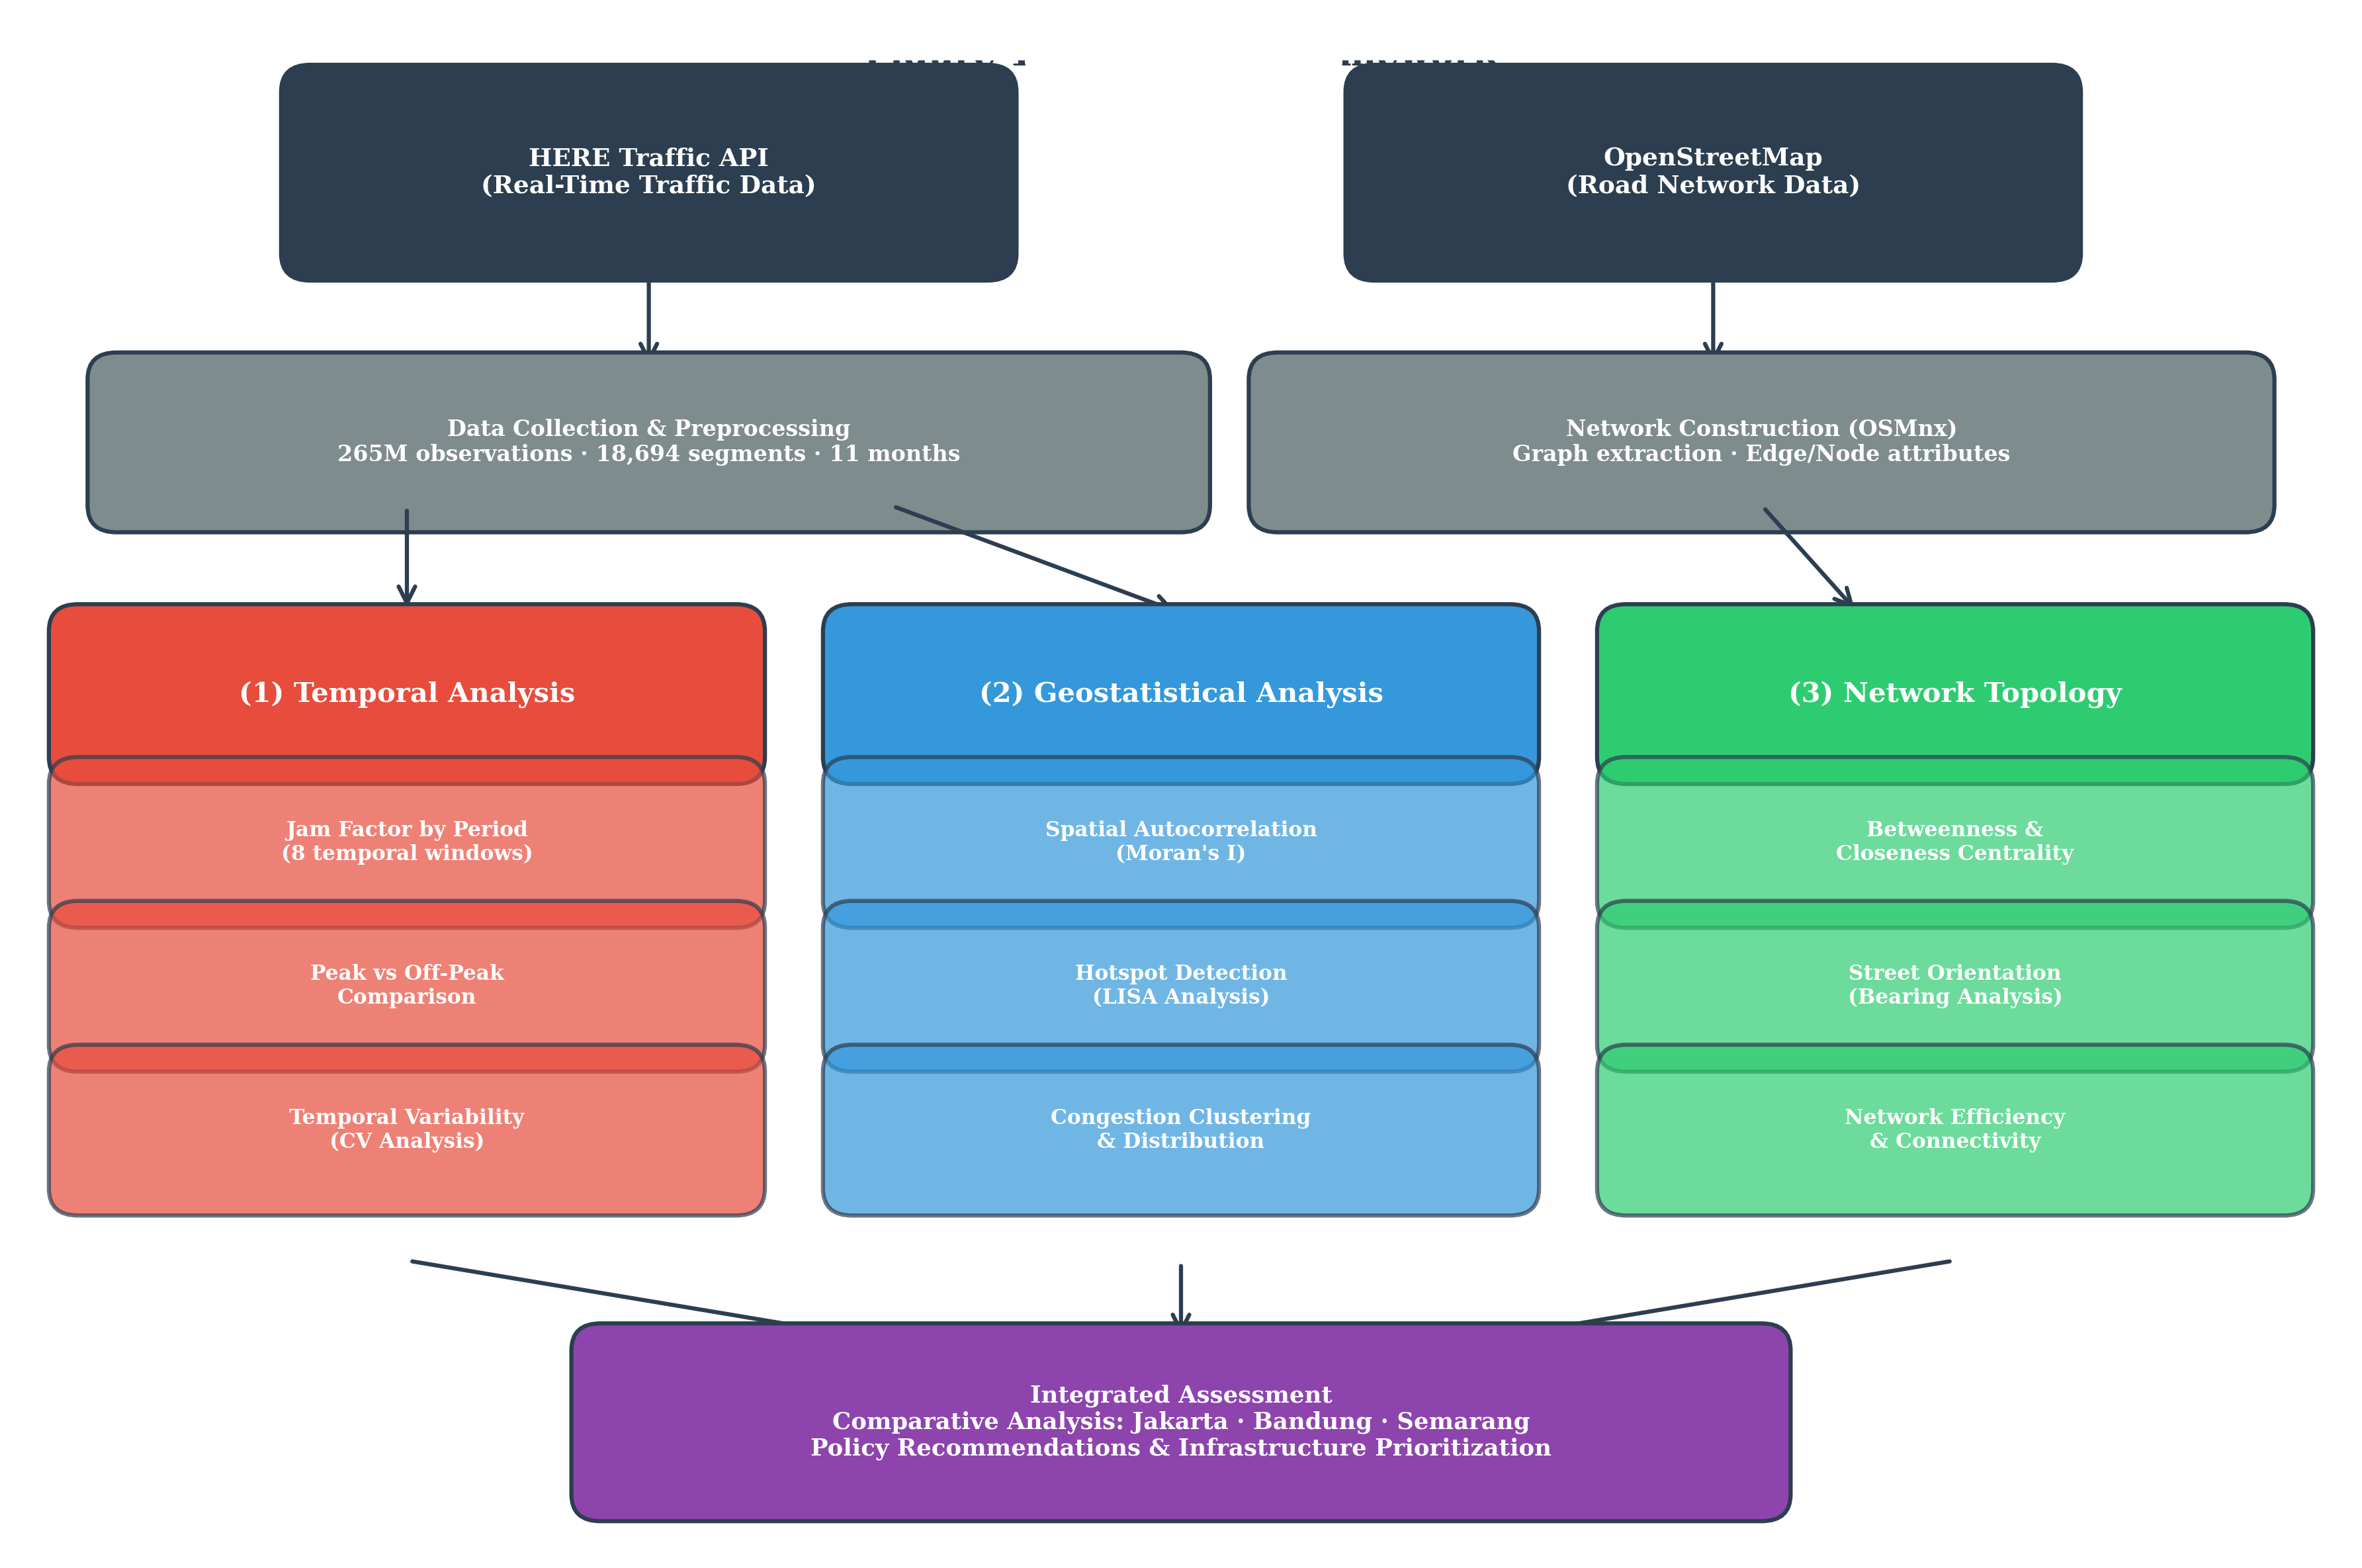
\includegraphics[width=\textwidth]{../figures/analytical_framework.png}
\caption{Analytical framework integrating temporal analysis, geostatistical methods, and network topology assessment}
\label{fig:fig1_analytic}
\end{figure}

\subsection{Temporal Pattern Analysis}

Temporal patterns were examined by calculating summary statistics for each period across all road segments. One-way ANOVA tested for significant differences between periods, with post-hoc Tukey HSD tests identifying specific significant pairs. To validate that temporal effects are not an artifact of jam factor normalization, ANOVA was also conducted on absolute speed (km/h), speed reduction (free-flow minus current speed, km/h), and free-flow speed, enabling cross-metric comparison of effect sizes ($\eta^2$).

\subsection{Geostatistical Analysis}

\paragraph{Global Spatial Autocorrelation}

Spatial autocorrelation was assessed using Moran's I \citep{Moran1950}:

\[I = \frac{n}{\sum_i \sum_j w_{ij}} \cdot \frac{\sum_i \sum_j w_{ij}(x_i - \bar{x})(x_j - \bar{x})}{\sum_i (x_i - \bar{x})^2}\]

where $n$ is the number of spatial units, $w_{ij}$ is the spatial weight between units $i$ and $j$, and $x_i$ is the jam factor at unit $i$. Spatial weights used K-nearest neighbors (k=8) based on segment centroids, preferred over queen contiguity for linear road segment geometries.

\paragraph{Local Indicators of Spatial Association}

Local Moran's I \citep{Anselin1995} identified hotspot and coldspot clusters:

\[I_i = \frac{(x_i - \bar{x})}{\sigma^2} \sum_j w_{ij}(x_j - \bar{x})\]

LISA was computed with KNN (k=8) weights, 999 random permutations, and Benjamini-Hochberg FDR correction. Segments were classified as HH (hotspot), LL (coldspot), or spatial outliers (HL/LH). Temporal stability was assessed via coefficient of variation: $CV = (\sigma/\mu) \times 100\%$.

\subsection{Spatial Scale Sensitivity Analysis (H3 Hexagonal Aggregation)}
\label{sec:method_h3}

A persistent methodological concern in urban spatial analysis is the modifiable areal unit problem (MAUP; \citealp{Openshaw1984}): statistical relationships can change substantially depending on the spatial unit chosen for analysis. Road segments vary in length from under 200\,m to over 3\,km, and predictors such as POI density and network centrality may operate at a neighbourhood rather than a segment scale. To test whether null correlations at the road-segment level reflect genuine absence of relationships or a unit-of-analysis artefact, we aggregated all variables into regular hexagonal bins using the Uber H3 hierarchical geospatial indexing system \citep{Brodsky2018} and re-ran the full correlation and spatial autocorrelation suite.

\textbf{Choice of hexagonal grid.} Hexagons are preferred over square grids for spatial aggregation because all six neighbours share an equal centroid-to-centroid distance, minimising directional bias in spatial weight matrices \citep{Sahr2003}. H3's hierarchical structure allows analysis at multiple scales using a consistent topology. Two resolutions were selected to span the neighbourhood and block scales relevant to urban traffic dynamics:

\begin{itemize}
  \item \textbf{Resolution 8}: mean hex diameter $\approx$461\,m, area $\approx$0.46\,km$^2$ (neighbourhood scale; 235--1,836 hexagons per city)
  \item \textbf{Resolution 9}: mean hex diameter $\approx$174\,m, area $\approx$0.10\,km$^2$ (block scale; 490--5,319 hexagons per city)
\end{itemize}

\textbf{Variable aggregation.} Each road segment centroid was assigned to its containing H3 cell using \texttt{h3.latlng\_to\_cell()}. Jam factor per hexagon was computed as the observation-weighted mean across all segments and all eight temporal periods within the cell:

\[\overline{JF}_{\text{hex}} = \frac{\displaystyle\sum_{s \in \text{hex}} \sum_{t} JF_{s,t} \cdot n_{s,t}}{\displaystyle\sum_{s \in \text{hex}} \sum_{t} n_{s,t}}\]

where $s$ indexes road segments, $t$ indexes temporal periods, $JF_{s,t}$ is the mean jam factor for segment $s$ in period $t$, and $n_{s,t}$ is the corresponding observation count. POI count per hexagon was the number of OSM POI centroids falling within each cell. Mean betweenness centrality per hexagon was the arithmetic mean of all OSM edge centrality values whose midpoints fell within the cell.

\textbf{Statistical tests.} Pearson and Spearman correlations were computed between hex-level jam factor and each predictor variable. Global Moran's I was computed using Queen contiguity weights derived from hexagon polygon adjacency---geometrically well-defined for regular hexagons, where each interior cell has exactly six neighbours---with row-standardisation and 999 random permutations for inference. Results are reported alongside the corresponding segment-level baseline values to quantify the effect of spatial scale on each statistic.

\subsection{Network Centrality Analysis}

Following \citet{Boeing2017}, we computed two network centrality metrics. \textbf{Betweenness centrality} measures the fraction of shortest paths passing through each edge:

\[C_B(e) = \sum_{s \neq t} \frac{\sigma_{st}(e)}{\sigma_{st}}\]

\textbf{Closeness centrality} measures average distance to all other nodes:

\[C_C(v) = \frac{n-1}{\sum_{u \neq v} d(u,v)}\]

Edge betweenness was computed on undirected networks weighted by edge length, with approximate sampling (k=500 source nodes) for large networks.

\subsection{Multilevel Variance Decomposition}

To provide a rigorous comparison of temporal and spatial variance contributions---avoiding the methodological asymmetry of comparing $\eta^2$ from categorical ANOVA against $R^2$ from continuous predictors---we fit a series of linear mixed-effects models with absolute speed (km/h) as the dependent variable. Speed was chosen over jam factor because it is not normalized to free-flow speed, eliminating the circularity concern.

Three nested models were estimated using restricted maximum likelihood (REML) via \texttt{statsmodels.mixedlm}:

\begin{enumerate}
  \item \textbf{Null model}: $\text{speed}_{it} = \gamma_0 + u_i + \varepsilon_{it}$, where $u_i \sim N(0, \sigma^2_u)$ is a random intercept for segment $i$. The intraclass correlation coefficient (ICC $= \sigma^2_u / (\sigma^2_u + \sigma^2_\varepsilon)$) partitions total speed variance into between-segment (spatial) and within-segment (temporal + residual) components.
  \item \textbf{Temporal model}: adds time period as a fixed effect. The pseudo-$R^2$ is the proportional reduction in residual variance relative to the null model, quantifying how much within-segment speed variation is explained by time of day.
  \item \textbf{Full model}: adds betweenness centrality and free-flow speed as segment-level (Level~2) predictors. The incremental $\Delta R^2$ is the proportional reduction in between-segment variance relative to the temporal model, quantifying how much spatial speed variation is explained by network topology and road capacity.
\end{enumerate}

This framework replaces the $\eta^2$ vs.\ $R^2$ comparison with a proper multilevel decomposition that accounts for the nested data structure (time periods within segments).

\subsection{Bottleneck and Capacity Drop Analysis}
\label{sec:bottleneck}

To determine if physical capacity constraints cause congestion, we created a multi-scale framework. Road segments received ordinal capacity scores (1--6) based on OSM highway classifications: motorway (6) through tertiary (2), with link variants scoring half their parent. Networks were filtered to include only HERE-comparable road types before analysis.

\paragraph{Graph-Based Capacity Drop Detection}

Capacity drops---where the road hierarchy decreases along the travel direction---were identified using the directed network graph. For each node, we compared the maximum capacity scores of incoming and outgoing edges.

\[\text{Drop ratio} = \frac{C_{\text{in}} - C_{\text{out}}}{C_{\text{in}}}\]

Nodes with a drop ratio of  $\geq$ 0.20 were classified as capacity drop locations. The Euclidean distance from each traffic segment to the nearest drop was calculated.

\paragraph{Local Bottleneck Gradient and Statistical Testing}

A local bottleneck gradient used K=10 nearest network neighbors per segment: segments with lower capacity than at least one neighbor were classified as ``local bottleneck,'' while others were classified as ``non-bottleneck.'' Three complementary tests assessed the capacity--congestion relationship: (1) a two-sample t-test comparing high- versus low-capacity road segments (Cohen's d); (2) Pearson and Spearman correlations between distance-to-nearest-drop and jam factor, plus a median-split t-test; and (3) a t-test comparing local bottleneck versus non-bottleneck segments.

\subsection{Open-Source Analysis Pipeline}
\label{sec:pipeline}

All analyses were implemented in a modular, open-source Python package (\texttt{pip install traffic-congestion-pipeline}; source: \url{https://github.com/firmanhadi21/traffic-analyses}; MIT licence). The package comprises approximately 6,700 lines of code organized into four stages: (1) Python-native HERE Traffic API data collection at configurable intervals; (2) large-scale aggregation using MD5-hashed geometry matching across 42,000+ GeoPackage files; (3) the full analytical workflow described above, with network centrality offloaded via SLURM to HPC resources; and (4) reproducible manuscript generation, where any change to analysis results propagates automatically to figures, tables, and the compiled PDF. Core dependencies include GeoPandas, OSMnx 2.0, NetworkX, PySAL (esda, libpysal, spreg), h3, SciPy, and statsmodels. The pipeline is city-agnostic: adding a new city requires only a bounding-box polygon and a HERE API key.



\section{Results}

\subsection{Overall Congestion Characteristics}

Table~\ref{tab:table5_congestion} presents summary statistics across all temporal periods. Jakarta exhibits the highest congestion: during the evening peak, 53.5\% of segments reach moderate congestion (JF > 2.0), compared with 11.9\% in Bandung and none in Semarang.

\FloatBarrier
\clearpage

\begin{longtable}[]{@{}llll@{}}
\caption{Congestion summary statistics by city (all temporal periods)}\label{tab:table5_congestion}\\
\toprule\noalign{}
Statistic & Jakarta & Bandung & Semarang \\
\midrule\noalign{}
\endhead
\bottomrule\noalign{}
\endlastfoot
Mean Jam Factor & 1.43 & 1.36 & 1.19 \\
Std. Deviation & 0.47 & 0.50 & 0.40 \\
Median & 1.63 & 1.52 & 1.34 \\
Max Segment Mean & 2.25 & 2.29 & 1.98 \\
Moderate+ congestion (evening peak) & 53.5\% & 11.9\% & 0.0\% \\
\end{longtable}
\FloatBarrier

\subsection{Temporal Patterns}

\paragraph{Period-Based Analysis}

Figure~\ref{fig:fig2_meanjam} and Table~\ref{tab:table6_meanjam} present mean jam factors by temporal period. The evening peak (16:00--19:00) shows the highest congestion across all cities---approximately 40\% above daily averages (39--41\%). All cities follow the same diurnal progression: minimal congestion at night (JF $\approx$ 0.5), rising through the morning peak, sustained at midday, and culminating in the evening peak before declining.

\begin{figure}
\centering
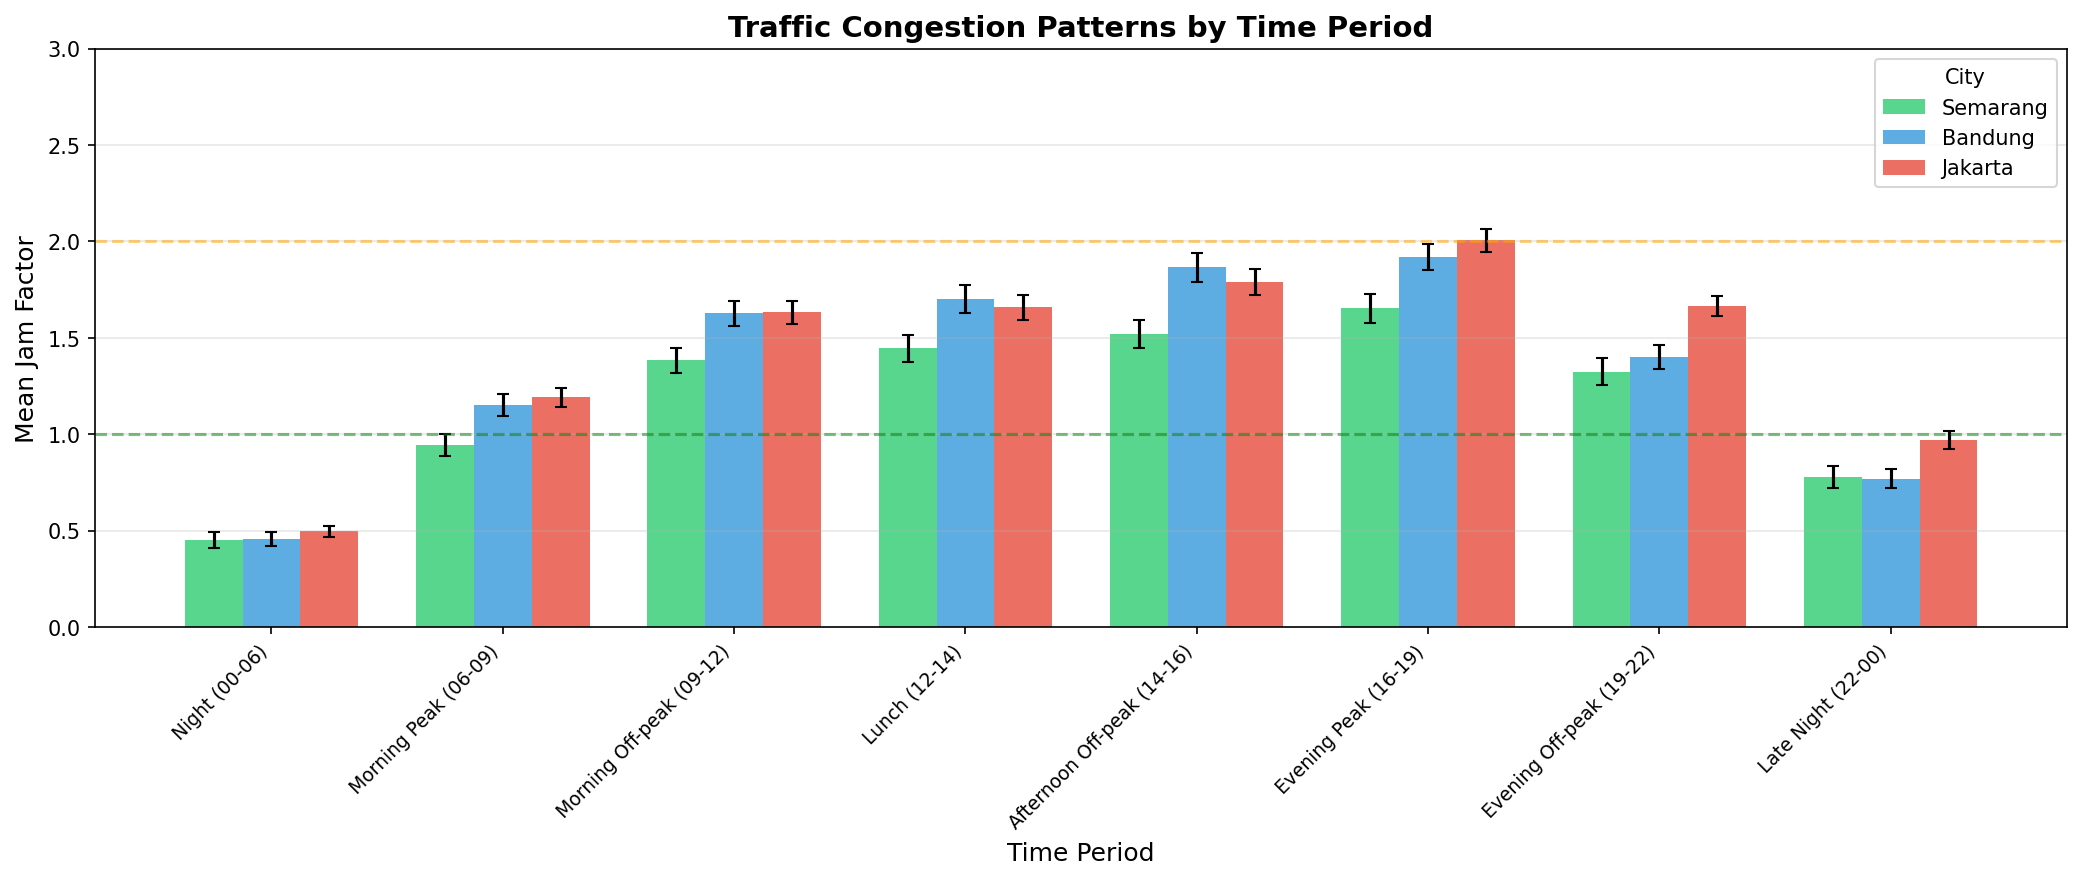
\includegraphics[width=\textwidth]{../figures/temporal_pattern_comparison.png}
\caption{Mean jam factor by temporal period across three cities}
\label{fig:fig2_meanjam}
\end{figure}

\begin{longtable}[]{@{}llll@{}}
\caption{Mean jam factor by temporal period}\label{tab:table6_meanjam}\\
\toprule\noalign{}
Period & Jakarta & Bandung & Semarang \\
\midrule\noalign{}
\endhead
\bottomrule\noalign{}
\endlastfoot
Night & 0.50 & 0.46 & 0.45 \\
Morning Peak & 1.19 & 1.15 & 0.95 \\
Morning Off-Peak & 1.63 & 1.63 & 1.39 \\
Lunch Hours & 1.66 & 1.70 & 1.45 \\
Afternoon Off-Peak & 1.79 & 1.87 & 1.52 \\
Evening Peak & \textbf{2.01} & \textbf{1.92} & \textbf{1.65} \\
Evening Off-Peak & 1.67 & 1.40 & 1.33 \\
Late Night & 0.97 & 0.77 & 0.78 \\
\end{longtable}

\paragraph{Statistical Significance of Temporal Variation}

One-way ANOVA confirms that temporal period differences are highly statistically significant (Table~\ref{tab:table_anova}). Post-hoc Tukey HSD tests reveal that all 28 pairwise period comparisons are significant (p < 0.05) for each city. The effect size ($\eta^2$) ranges from 8--10\% for jam factor and speed reduction, 5--6\% for absolute speed, and effectively zero for free-flow speed (Table~\ref{tab:speed_validation}). The similarity of $\eta^2$ values between jam factor (8--9\%) and speed reduction (8--10\%) confirms that temporal dominance is not an artifact of jam factor normalization: the same temporal pattern appears in absolute speed metrics. Free-flow speed shows no temporal variation, as expected since it reflects road design capacity. Weekday congestion exceeds weekend levels by approximately 35--40\%, with Friday evenings peaking and Sunday mornings at a minimum.

\begin{longtable}[]{@{}llll@{}}
\caption{ANOVA results for temporal period effects}\label{tab:table_anova}\\
\toprule\noalign{}
City & F-statistic & p-value & Significant Period Pairs \\
\midrule\noalign{}
\endhead
\bottomrule\noalign{}
\endlastfoot
Jakarta & 1,191,699.66 & < 0.001 & 28/28 \\
Bandung & 224,445.67 & < 0.001 & 28/28 \\
Semarang & 45,863.33 & < 0.001 & 28/28 \\
\end{longtable}

\begin{longtable}[]{@{}lllll@{}}
\caption{Temporal variance explained ($\eta^2$) by metric type}\label{tab:speed_validation}\\
\toprule\noalign{}
City & Jam factor & Current speed & Speed reduction & Free-flow speed \\
\midrule\noalign{}
\endhead
\bottomrule\noalign{}
\endlastfoot
Semarang & 8.8\% & 5.1\% & 9.6\% & $<$0.01\% \\
Bandung & 9.4\% & 5.9\% & 8.8\% & $<$0.01\% \\
Jakarta & 8.2\% & 5.2\% & 8.2\% & $<$0.01\% \\
\end{longtable}

\subsection{Spatial Pattern Analysis}

\paragraph{Global Spatial Autocorrelation}

Global Moran's I (KNN k=8 weights) is close to zero and non-significant for all cities (Table~\ref{tab:table_moran}), indicating no strong overall spatial autocorrelation throughout the entire study period. Results are consistent across different weight settings (KNN k=4, k=12; distance bands 500m and 1000m), and calculating Moran's I separately for each temporal period also produced non-significant results across all cities and periods (all p > 0.05). This confirms that the null global autocorrelation finding is not an artifact of temporal averaging or weight specification. A spatial scale-sensitivity analysis using Uber H3 hexagonal aggregation 
(Section~\ref{sec:h3_robustness}) further confirms this null result for Semarang and Bandung, while revealing a weak but statistically significant neighbourhood-level autocorrelation for Jakarta ($I = 0.030$, $p = 0.033$ at resolution~8) not detectable at the road-segment level.

\FloatBarrier
\begin{longtable}[]{@{}lllll@{}}
\caption{Global spatial autocorrelation statistics (Moran's I)}\label{tab:table_moran}\\
\toprule\noalign{}
City & Moran's I & Z-score & p-value & Interpretation \\
\midrule\noalign{}
\endhead
\bottomrule\noalign{}
\endlastfoot
Jakarta & 0.0026 & 0.69 & 0.492 & Random \\
Bandung & 0.0075 & 0.93 & 0.353 & Random \\
Semarang & -0.0039 & -0.21 & 0.837 & Random \\
\end{longtable}
\FloatBarrier

\paragraph{Local Hotspot Identification}

Despite weak global autocorrelation, LISA identifies meaningful local clusters (Table~\ref{tab:table_lisa}). Approximately 10\% of segments in Jakarta and Bandung participate in significant clusters (7.2\% in Semarang). After Benjamini-Hochberg FDR correction, no segments remain significant, indicating that while observed clusters exceed chance expectations by approximately 2$\times$, individual p-values are not sufficiently small to survive multiple testing correction. Uncorrected LISA results should therefore be interpreted as suggestive of local clustering tendencies; the patterns are geographically coherent (concentrated along known corridors) and exceed chance expectations by $\sim$2$\times$, suggesting genuine but weak local spatial structure. Getis-Ord Gi* analysis corroborates LISA: 9--10\% of segments are classified as significant hot or cold spots, with cold spots slightly outnumbering hot spots across all cities.

\begin{longtable}[]{@{}
  >{\raggedright\arraybackslash}p{(\linewidth - 6\tabcolsep) * \real{0.3333}}
  >{\raggedleft\arraybackslash}p{(\linewidth - 6\tabcolsep) * \real{0.2143}}
  >{\raggedleft\arraybackslash}p{(\linewidth - 6\tabcolsep) * \real{0.2143}}
  >{\raggedleft\arraybackslash}p{(\linewidth - 6\tabcolsep) * \real{0.2381}}@{}}
\caption{LISA cluster classification (evening peak, $p < 0.05$)}\label{tab:table_lisa}\\
\toprule\noalign{}
Cluster Type & Jakarta & Bandung & Semarang \\
\midrule\noalign{}
\endhead
\bottomrule\noalign{}
\endlastfoot
HH (Hotspot) & 438 (3.0\%) & 86 (2.8\%) & 19 (1.8\%) \\
LL (Coldspot) & 347 (2.4\%) & 73 (2.4\%) & 23 (2.1\%) \\
HL (High-Low Outlier) & 334 (2.3\%) & 69 (2.2\%) & 19 (1.8\%) \\
LH (Low-High Outlier) & 416 (2.9\%) & 92 (3.0\%) & 17 (1.6\%) \\
Not Significant & 13,014 (89.5\%) & 2,749 (89.6\%) & 998 (92.8\%) \\
\textbf{Total Significant} & \textbf{1,535 (10.5\%)} & \textbf{320 (10.4\%)} & \textbf{78 (7.2\%)} \\
\end{longtable}

\textbf{Jakarta} hotspots concentrate in: the Sudirman-Thamrin CBD corridor; the Tangerang-Jakarta western approach; and the Bekasi-Jakarta eastern approach (Figure~\ref{fig:jkt_hotspots}). \textbf{Bandung} hotspots include the Dago/Setiabudhi northern corridors, Asia-Afrika city center, and Soekarno-Hatta eastern industrial zone (Supplementary Figure~S1). \textbf{Semarang} hotspots appear along Pandanaran/Pemuda central corridors, Siliwangi coastal road, and the Majapahit eastern approach (Supplementary Figure~S2).

\begin{figure}
\centering
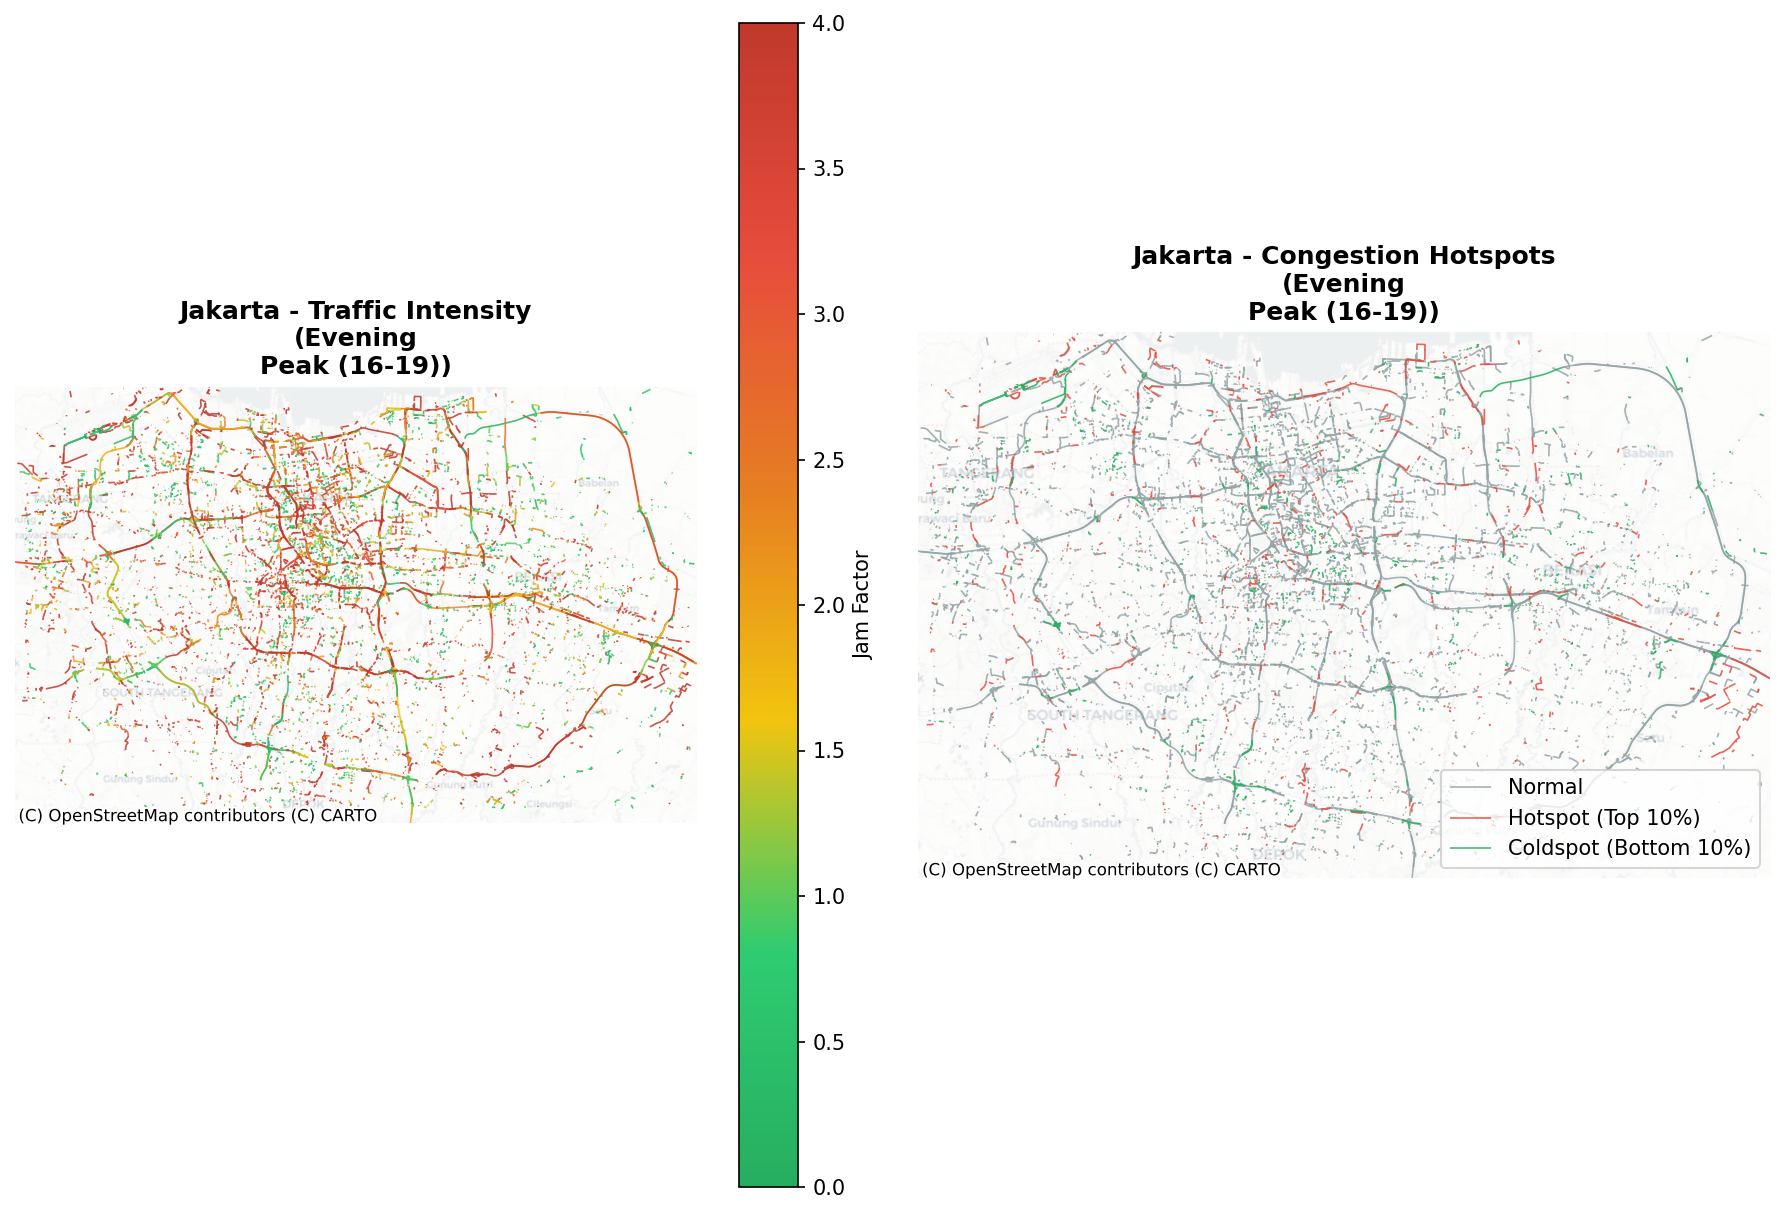
\includegraphics[width=\textwidth]{../figures/jkt_hotspots_evening_peak.png}
\caption{Spatial distribution of congestion hotspots --- Jakarta. Bandung and Semarang hotspot maps are provided in Supplementary Figures~S1--S2.}
\label{fig:jkt_hotspots}
\end{figure}

\subsection{Network Topology--Congestion Relationships}

\paragraph{Betweenness Centrality}

Traffic segments were spatially joined to OSMnx edges using centroid-based nearest-neighbor matching (200m threshold). Match quality is high: median centroid distances are under 20m, with over 85\% of matches within 50m. To test whether centrality--congestion correlations differ by metric type, we computed Pearson $R^2$ between betweenness centrality and four traffic metrics during the evening peak (Table~\ref{tab:centrality_speed}). The results reveal a striking pattern: centrality shows moderate correlations with jam factor ($R^2$ = 0.06--0.14) and speed reduction ($R^2$ = 0.07--0.13), but near-zero correlations with absolute current speed ($R^2$ < 0.003). This divergence arises because jam factor and speed reduction both incorporate free-flow speed normalization, while absolute speed does not. Free-flow speed itself shows weak positive correlation with centrality ($R^2$ = 0.02--0.05), reflecting that topologically important roads tend to have higher design speeds. Centrality's apparent ``effect'' on jam factor is thus largely mediated through its association with free-flow speed---a road characteristic---rather than through any direct influence on congestion severity.

\paragraph{Positive Control: Free-Flow Speed as Spatial Predictor}

To confirm that the near-zero centrality--congestion correlations are genuine rather than a methodological artefact, we tested whether our spatial data can detect \textit{known} spatial relationships. Free-flow speed---a road design characteristic determined by lane count, speed limit, and road class---should be strongly predicted by segment location. Indeed, free-flow speed explains 60--71\% of the variance in current speed across all cities ($R^2$ = 0.60 in Bandung, 0.66 in Jakarta, 0.71 in Semarang), confirming that the data and spatial matching procedure successfully capture between-segment differences. The contrast is stark: the same analytical pipeline that detects strong spatial structure in road design ($R^2 = 0.60$--$0.71$) finds no spatial structure in congestion ($R^2 < 0.003$). This positive control rules out insufficient statistical power, spatial matching errors, or data quality issues as explanations for the null congestion result.

\begin{longtable}[]{@{}lllll@{}}
\caption{Centrality--congestion correlations by metric type (Pearson $R^2$, evening peak)}\label{tab:centrality_speed}\\
\toprule\noalign{}
City & Jam factor & Current speed & Speed reduction & Free-flow speed \\
\midrule\noalign{}
\endhead
\bottomrule\noalign{}
\endlastfoot
Semarang (n=1,059) & 0.0835 & 0.0026 & 0.1083 & 0.0194 \\
Bandung (n=3,039) & 0.1355 & 0.0002 & 0.1298 & 0.0493 \\
Jakarta (n=14,453) & 0.0639 & 0.0009 & 0.0669 & 0.0309 \\
\end{longtable}

\begin{figure}
\centering
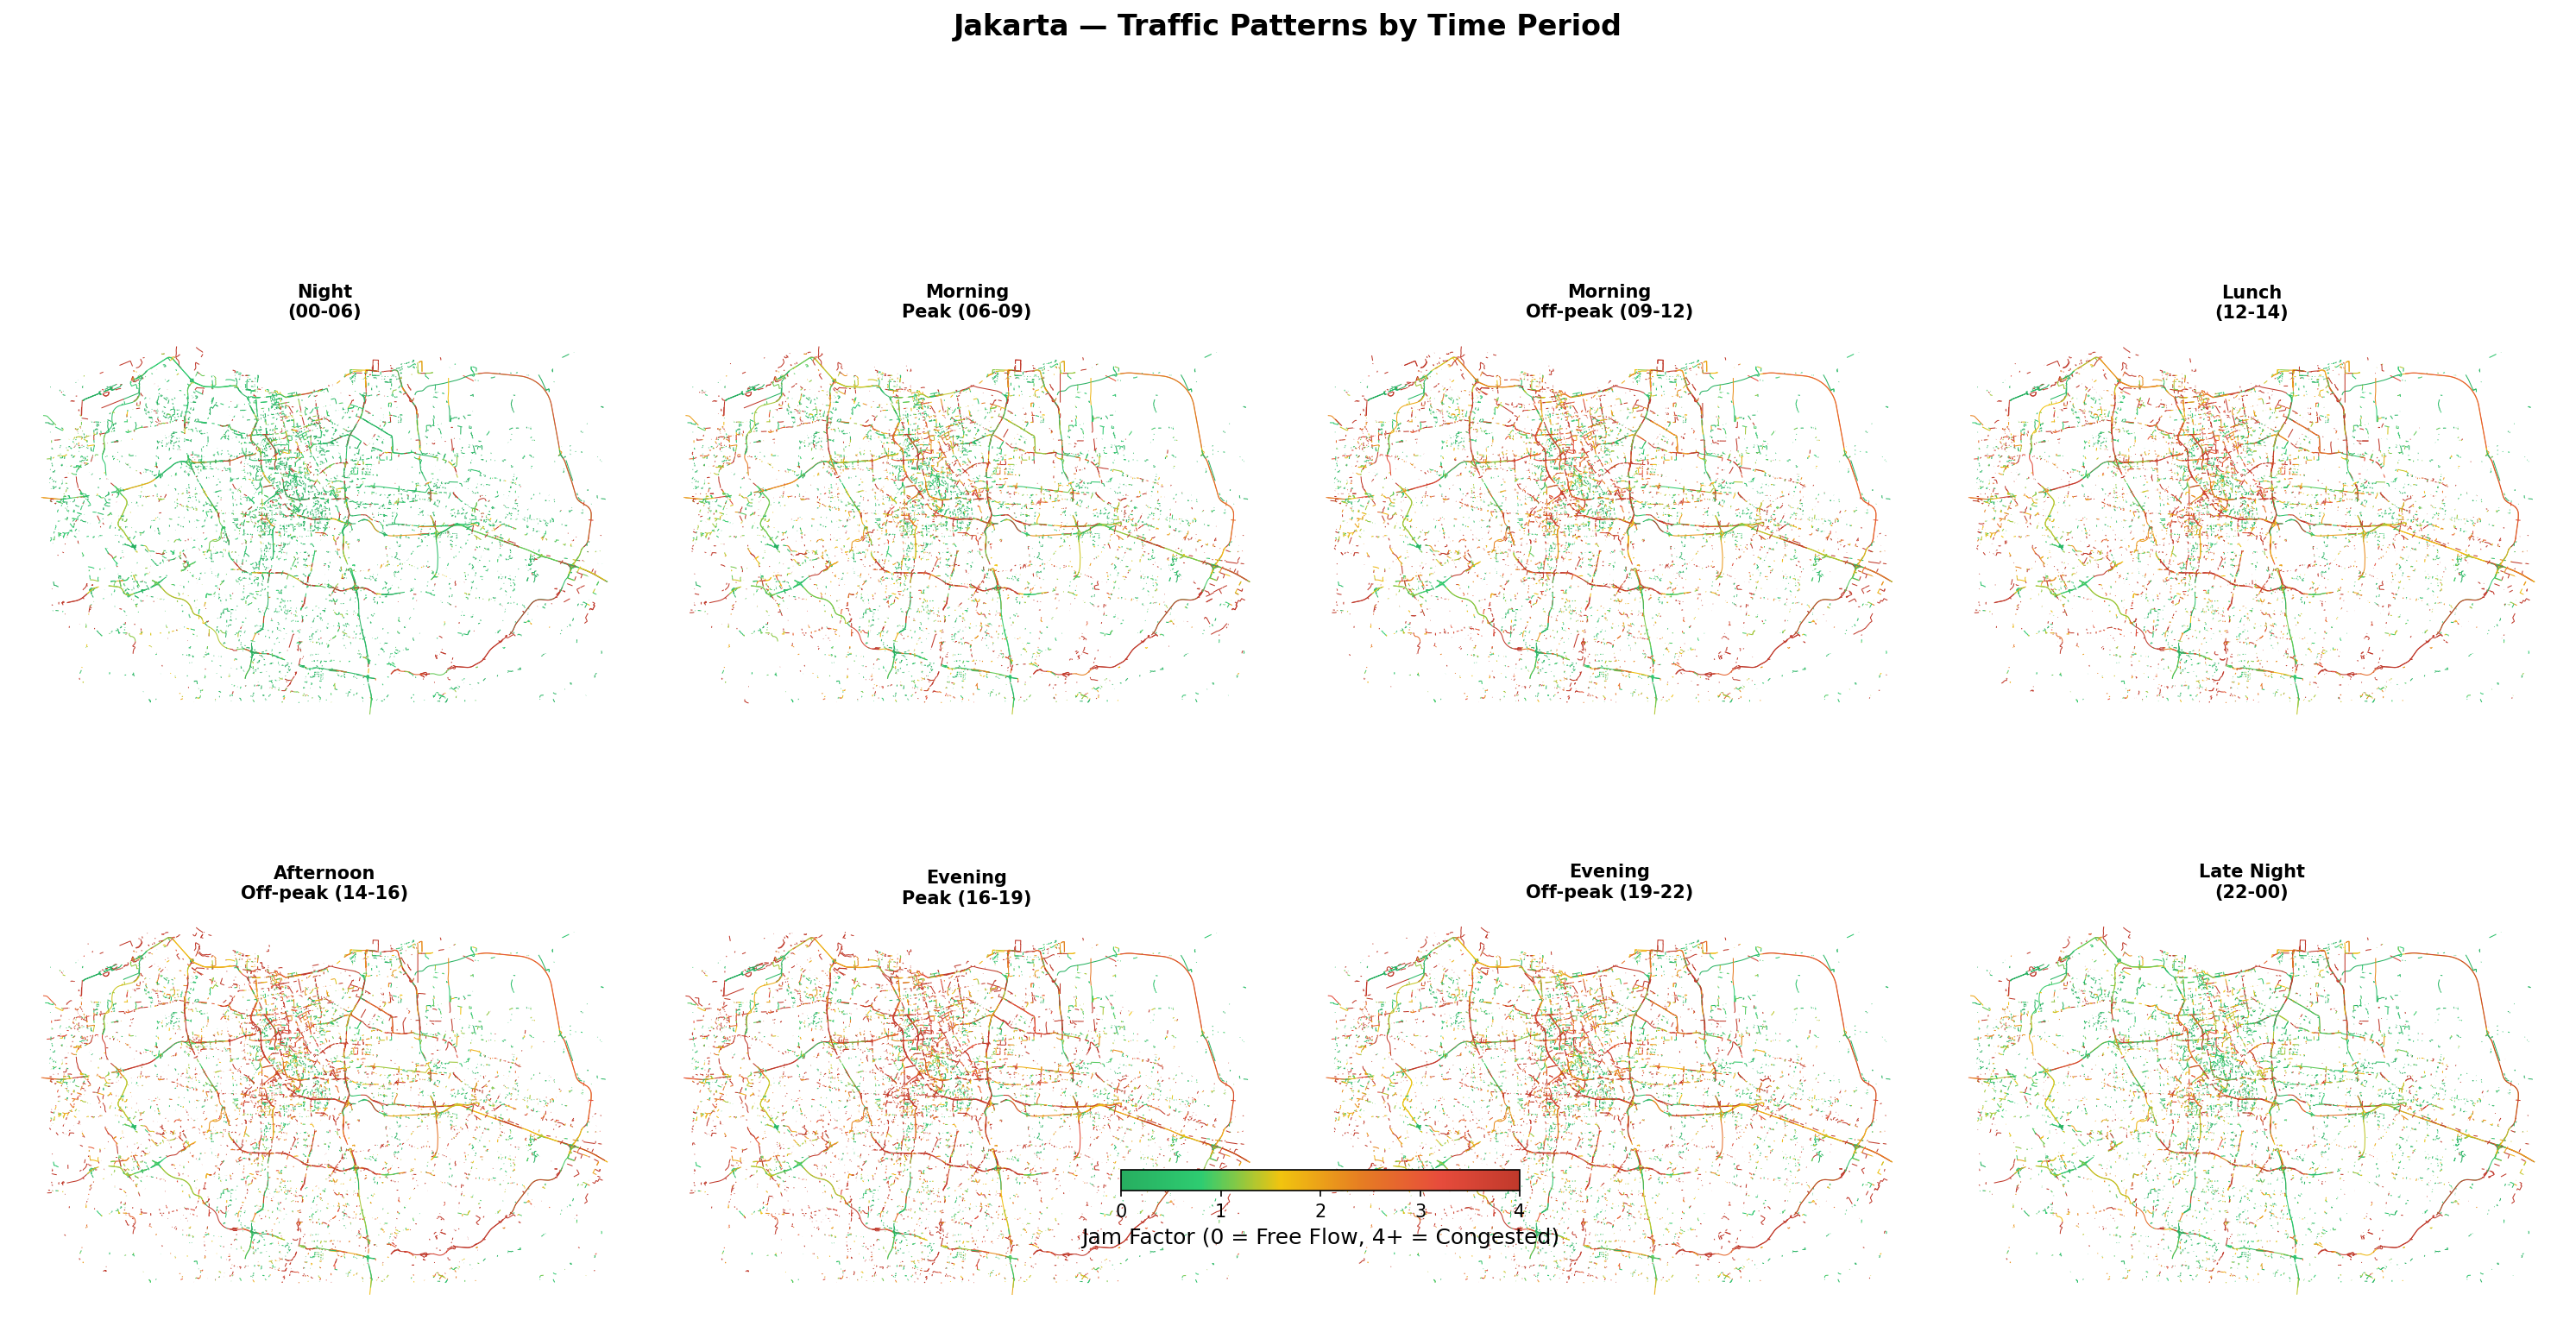
\includegraphics[width=\textwidth]{../figures/jkt_traffic_maps.png}
\caption{Edge betweenness centrality --- Jakarta}
\label{fig:jkt_centrality}
\end{figure}

\begin{figure}
\centering
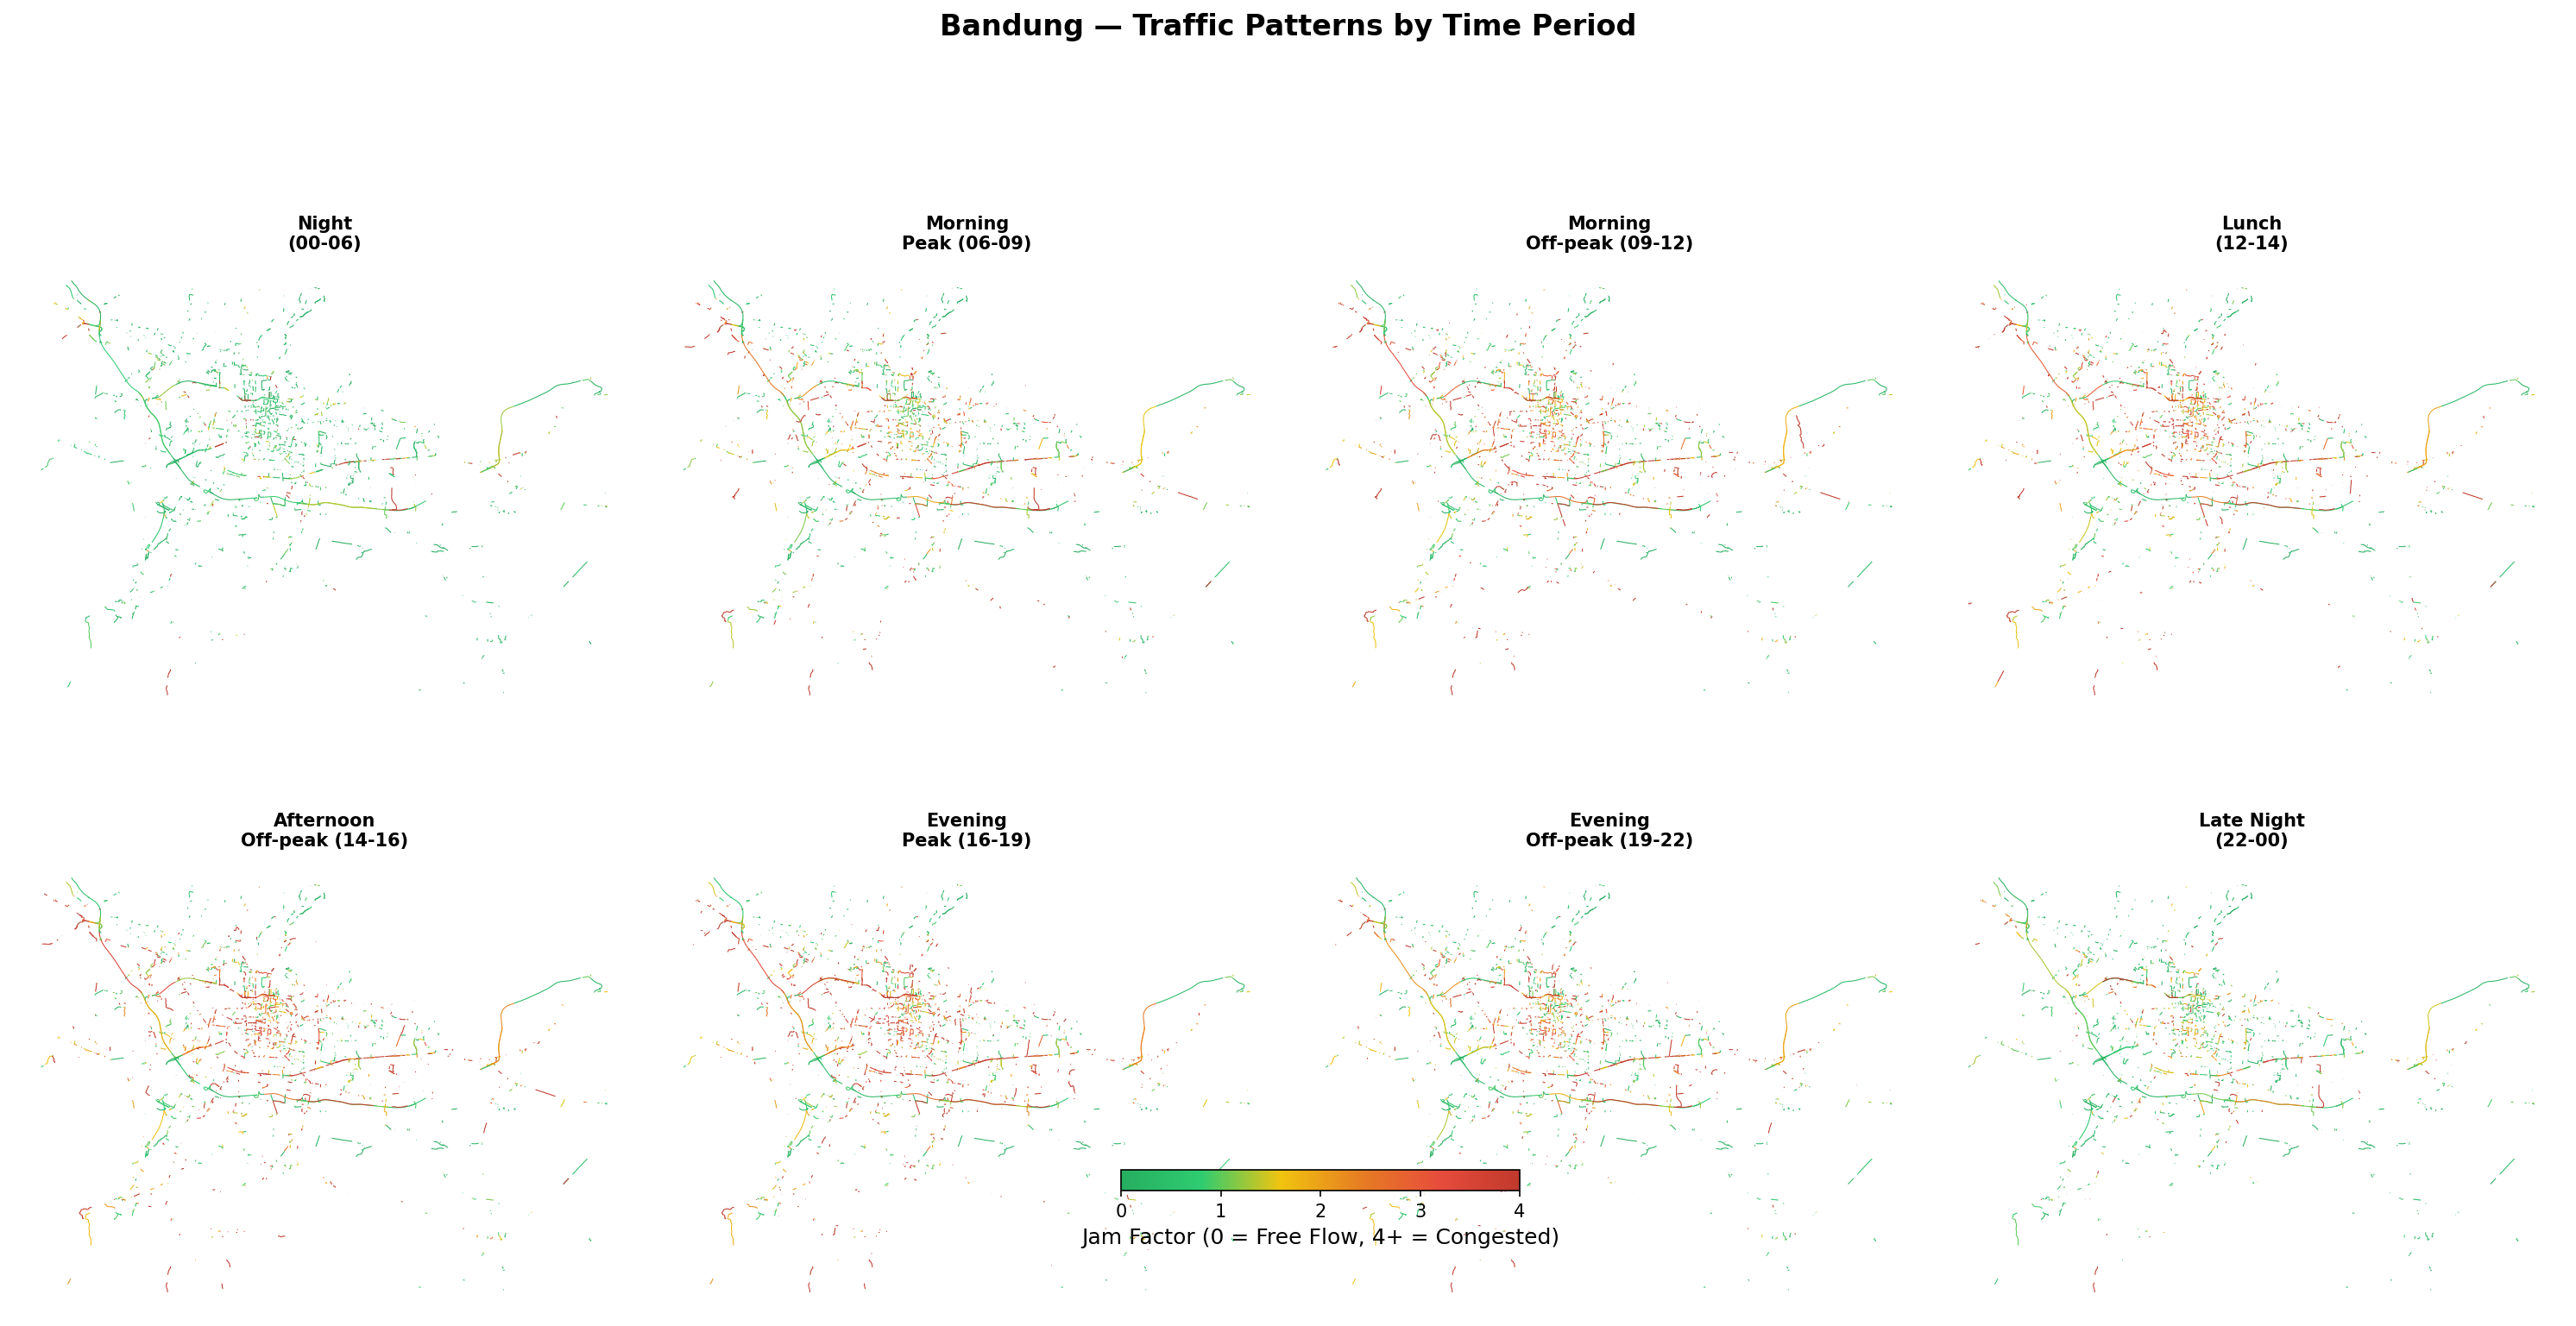
\includegraphics[width=\textwidth]{../figures/bdg_traffic_maps.png}
\caption{Edge betweenness centrality --- Bandung}
\label{fig:bdg_centrality}
\end{figure}

\begin{figure}
\centering
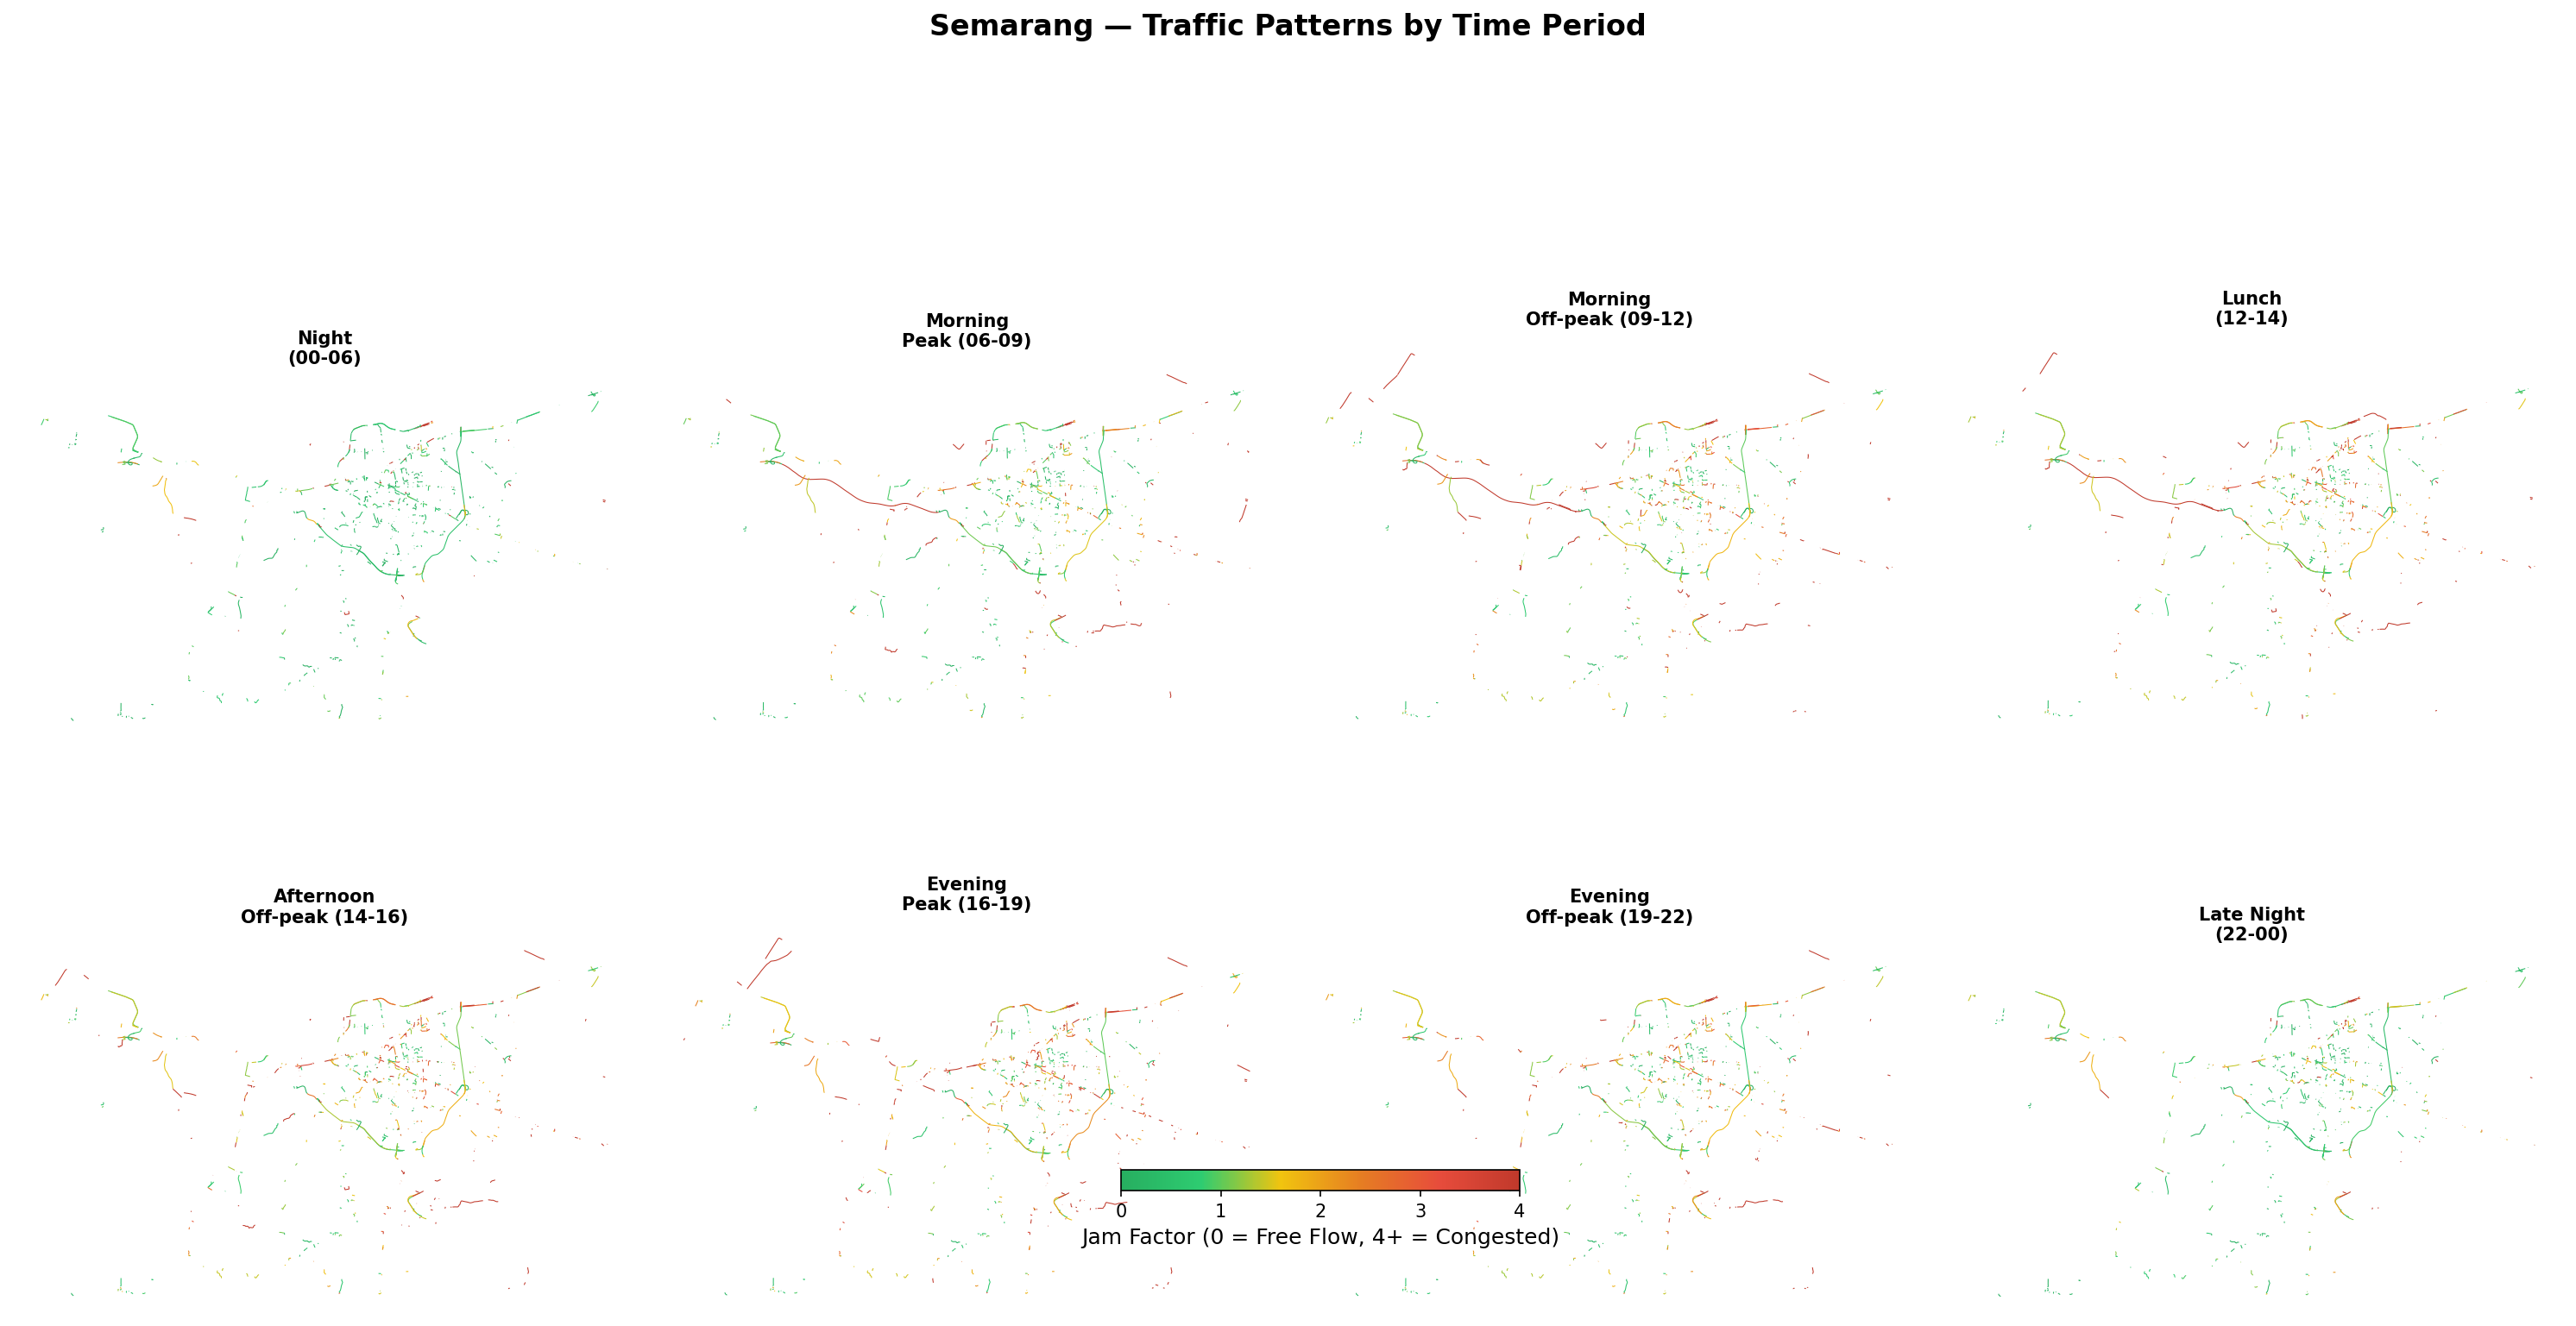
\includegraphics[width=\textwidth]{../figures/smg_traffic_maps.png}
\caption{Edge betweenness centrality --- Semarang}
\label{fig:smg_centrality}
\end{figure}

\FloatBarrier
\paragraph{POI Density Analysis}

Point of Interest density was computed using network-distance analysis (400m walking network distance, approximately a 5-minute walk; \citealp{Moudon2006}). Sensitivity analyses across 200m, 400m, 800m, and 1200m thresholds confirm results are robust. POI density shows \textbf{no meaningful correlation} with congestion (Table~\ref{tab:table11}).

Categorical comparison of high-POI activity centers (top quartile) versus peripheral areas (bottom quartile) confirms this: differences are negligible ($|d|$ < 0.05, p > 0.3) for all cities, demonstrating that congestion is location-independent. Spatial regression (OLS, Spatial Lag, and Spatial Error models) corroborates these results, with $R^2$ < 0.3\% across all specifications; accounting for spatial structure reveals no hidden centrality--congestion relationships.

\begin{longtable}[]{@{}llllll@{}}
\caption{POI density--congestion correlations}\label{tab:table11}\\
\toprule\noalign{}
City & Total POIs & Pearson r & p-value & Spearman $\rho$ & p-value \\
\midrule\noalign{}
\endhead
\bottomrule\noalign{}
\endlastfoot
Jakarta & 221,034 & -0.0005 & 0.954 & 0.0084 & 0.313 \\
Bandung & 56,844 & -0.0128 & 0.478 & 0.0053 & 0.768 \\
Semarang & 18,937 & -0.0072 & 0.814 & -0.0124 & 0.685 \\
\end{longtable}

\subsection{Robustness Check: Spatial Scale Sensitivity}
\label{sec:h3_robustness}

To address the potential modifiable areal unit problem (MAUP)---the possibility that null correlations reflect a mismatch between the road-segment unit of analysis and the neighbourhood scale at which POI density and network centrality actually operate---we re-ran all spatial correlations after aggregating variables into Uber H3 hexagonal bins at two resolutions: resolution~8 (mean hex diameter $\approx$461\,m, area $\approx$0.46\,km$^2$, neighbourhood scale) and resolution~9 (diameter $\approx$174\,m, area $\approx$0.10\,km$^2$, block scale). For each hexagon, jam factor was computed as the observation-weighted mean across all road segments and temporal periods falling within the cell (235--1,836 hexagons per city at resolution~8; 490--5,319 at resolution~9). POI counts and mean edge betweenness centrality were aggregated to the same hexagonal grid using the same OSM data sources as the segment-level analyses.

POI-density and centrality correlations remained negligible at both resolutions across all three cities (all $|\rho| < 0.08$, all $p > 0.07$; Table~\ref{tab:h3_robustness}). The maximum observed effect was Semarang's POI Spearman $\rho$ = +0.077 ($p$ = 0.242) at resolution~8, still far below conventional significance thresholds and practically negligible in magnitude. These results confirm that the null segment-level findings reported above are not an artefact of spatial scale: POI density and network centrality do not predict congestion at any spatial grain tested, from individual road segments to 461\,m neighbourhood hexagons.

Global Moran's I on hex-aggregated jam factor was non-significant for Semarang and Bandung at both resolutions ($p > 0.05$), consistent with the segment-level finding. Jakarta, however, exhibited weak but statistically significant positive spatial autocorrelation at the neighbourhood scale at both resolutions ($I = 0.030$, $p = 0.033$ at resolution~8; $I = 0.022$, $p = 0.030$ at resolution~9), a pattern not detectable at the road-segment level ($I = 0.003$, $p = 0.492$). This suggests that Jakarta's congestion has coherent neighbourhood-level spatial structure---hexagons with elevated congestion tend to be surrounded by similarly elevated neighbours---but this clustering is not explained by POI density or betweenness centrality, both of which remain uncorrelated with congestion even within Jakarta at the hex scale. The drivers of this weak but consistent neighbourhood clustering in Jakarta warrant further investigation, with candidate explanatory variables including land-use mix, population density, and access to public transit.

\begin{longtable}[]{@{}llrlll@{}}
\caption{H3 hex-level robustness check --- Spearman $\rho$ and Global Moran's I (p-values in parentheses)}\label{tab:h3_robustness}\\
\toprule\noalign{}
City & Resolution & Hexagons & POI $\rho$ (p) & Centrality $\rho$ (p) & Moran's I (p) \\
\midrule\noalign{}
\endhead
\bottomrule\noalign{}
\endlastfoot
Semarang & 8 ($\approx$461\,m) & 235  & +0.077 (0.242) & +0.053 (0.427) & $-$0.081 (0.087) \\
Semarang & 9 ($\approx$174\,m) & 490  & +0.033 (0.462) & +0.022 (0.630) & +0.004 (0.443) \\
Bandung  & 8 ($\approx$461\,m) & 517  & +0.053 (0.228) & +0.041 (0.352) & +0.052 (0.055) \\
Bandung  & 9 ($\approx$174\,m) & 1,222 & +0.027 (0.339) & +0.053 (0.070) & $-$0.008 (0.412) \\
Jakarta  & 8 ($\approx$461\,m) & 1,836 & +0.021 (0.362) & $-$0.007 (0.784) & +0.030 (0.033)\textsuperscript{*} \\
Jakarta  & 9 ($\approx$174\,m) & 5,319 & $-$0.014 (0.314) & $-$0.003 (0.836) & +0.022 (0.030)\textsuperscript{*} \\
\end{longtable}

\textit{Segment-level baseline for comparison: POI $\rho$ < 0.013 (all $p$ > 0.6); Centrality $\rho$ < 0.012 (all $p$ > 0.44); Moran's I $<$ 0.008 (all $p$ > 0.35). \textsuperscript{*}$p$ < 0.05.}

\begin{figure}[htbp]
\centering
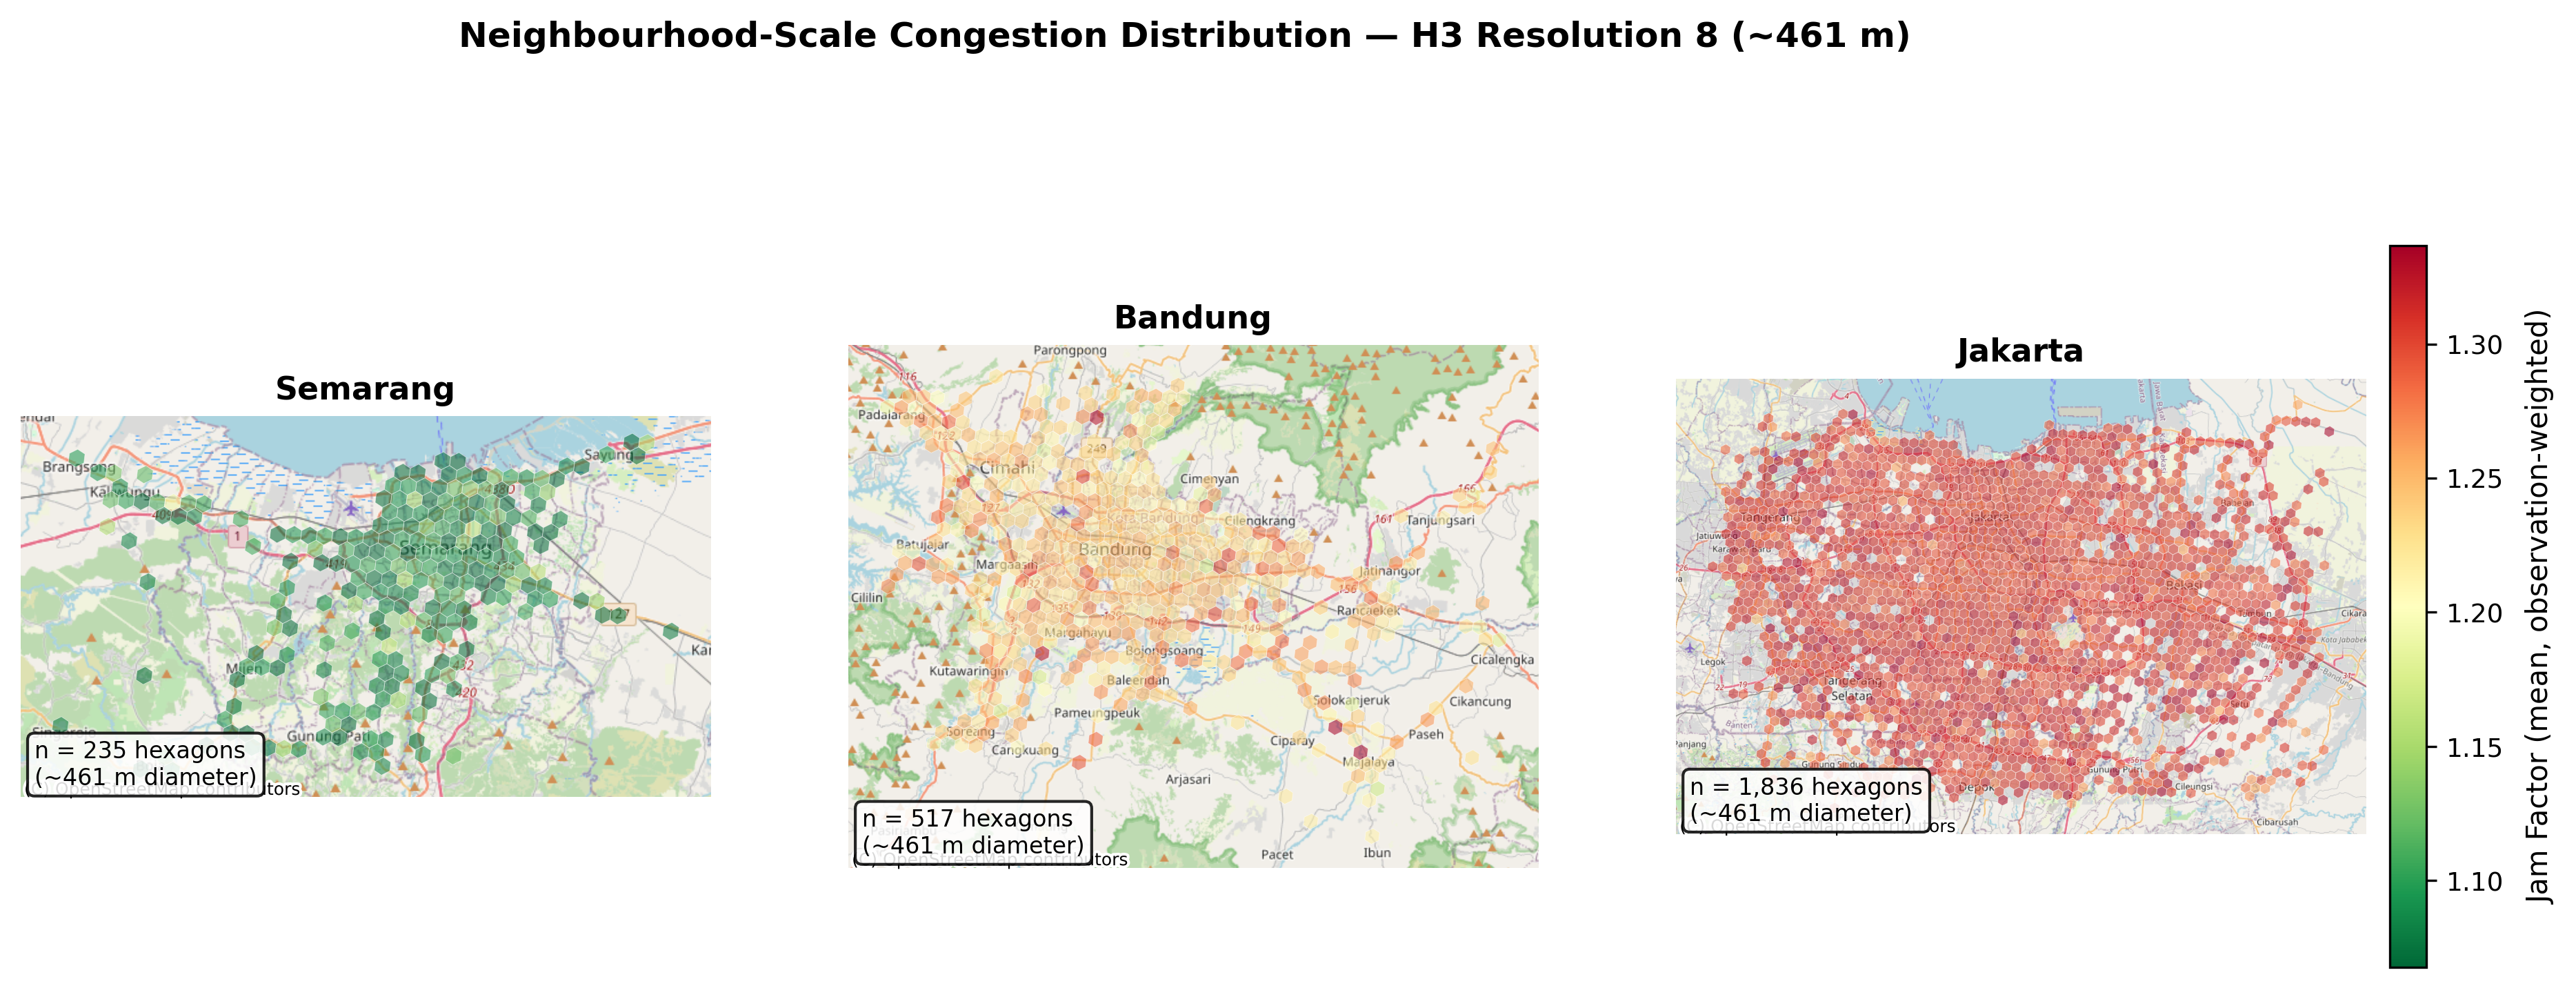
\includegraphics[width=\textwidth]{../figures/h3_congestion_maps.png}
\caption{Neighbourhood-scale congestion distribution at H3 resolution 8 ($\approx$461\,m hex diameter). Each hexagon shows the observation-weighted mean jam factor aggregated across all 8 temporal periods and all road segments within the cell. Jakarta's higher and more spatially structured congestion is visible relative to Bandung and Semarang.}
\label{fig:h3_congestion_maps}
\end{figure}

\begin{figure}[htbp]
\centering
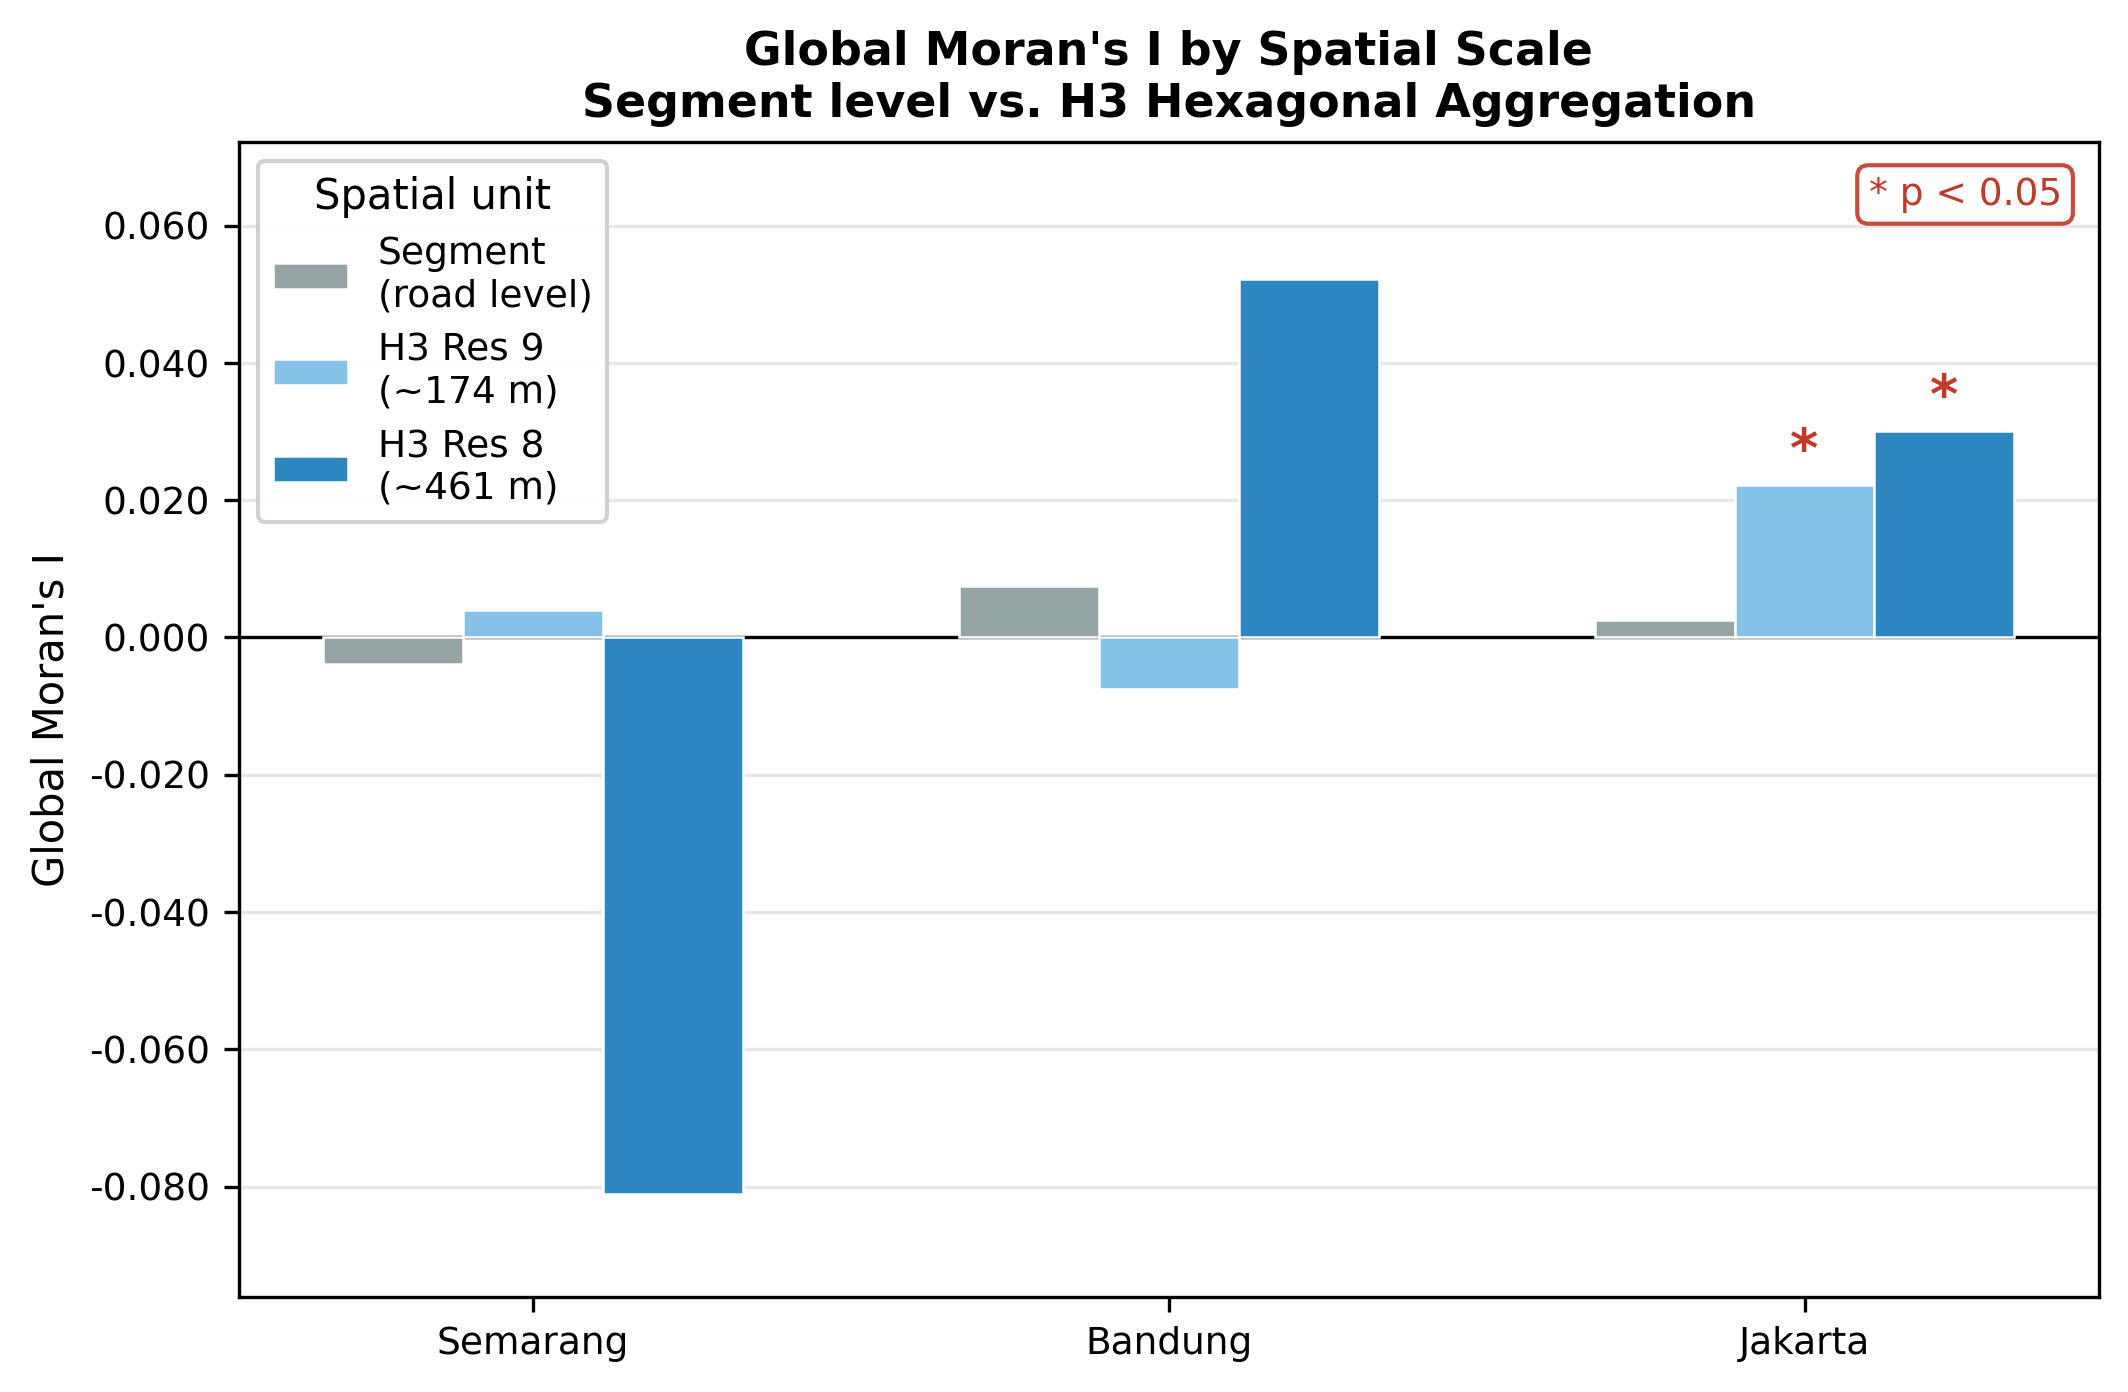
\includegraphics[width=0.75\textwidth]{../figures/h3_morans_scale.png}
\caption{Global Moran's I by spatial scale for three cities. Bars show Moran's I at the road-segment level, H3 resolution~9 ($\approx$174\,m), and H3 resolution~8 ($\approx$461\,m). Asterisk (*) denotes $p$ < 0.05. Jakarta's spatial autocorrelation reaches significance only at the hexagonal aggregation scales, while Semarang and Bandung remain statistically random at all three scales.}
\label{fig:h3_morans_scale}
\end{figure}

\begin{figure}[htbp]
\centering
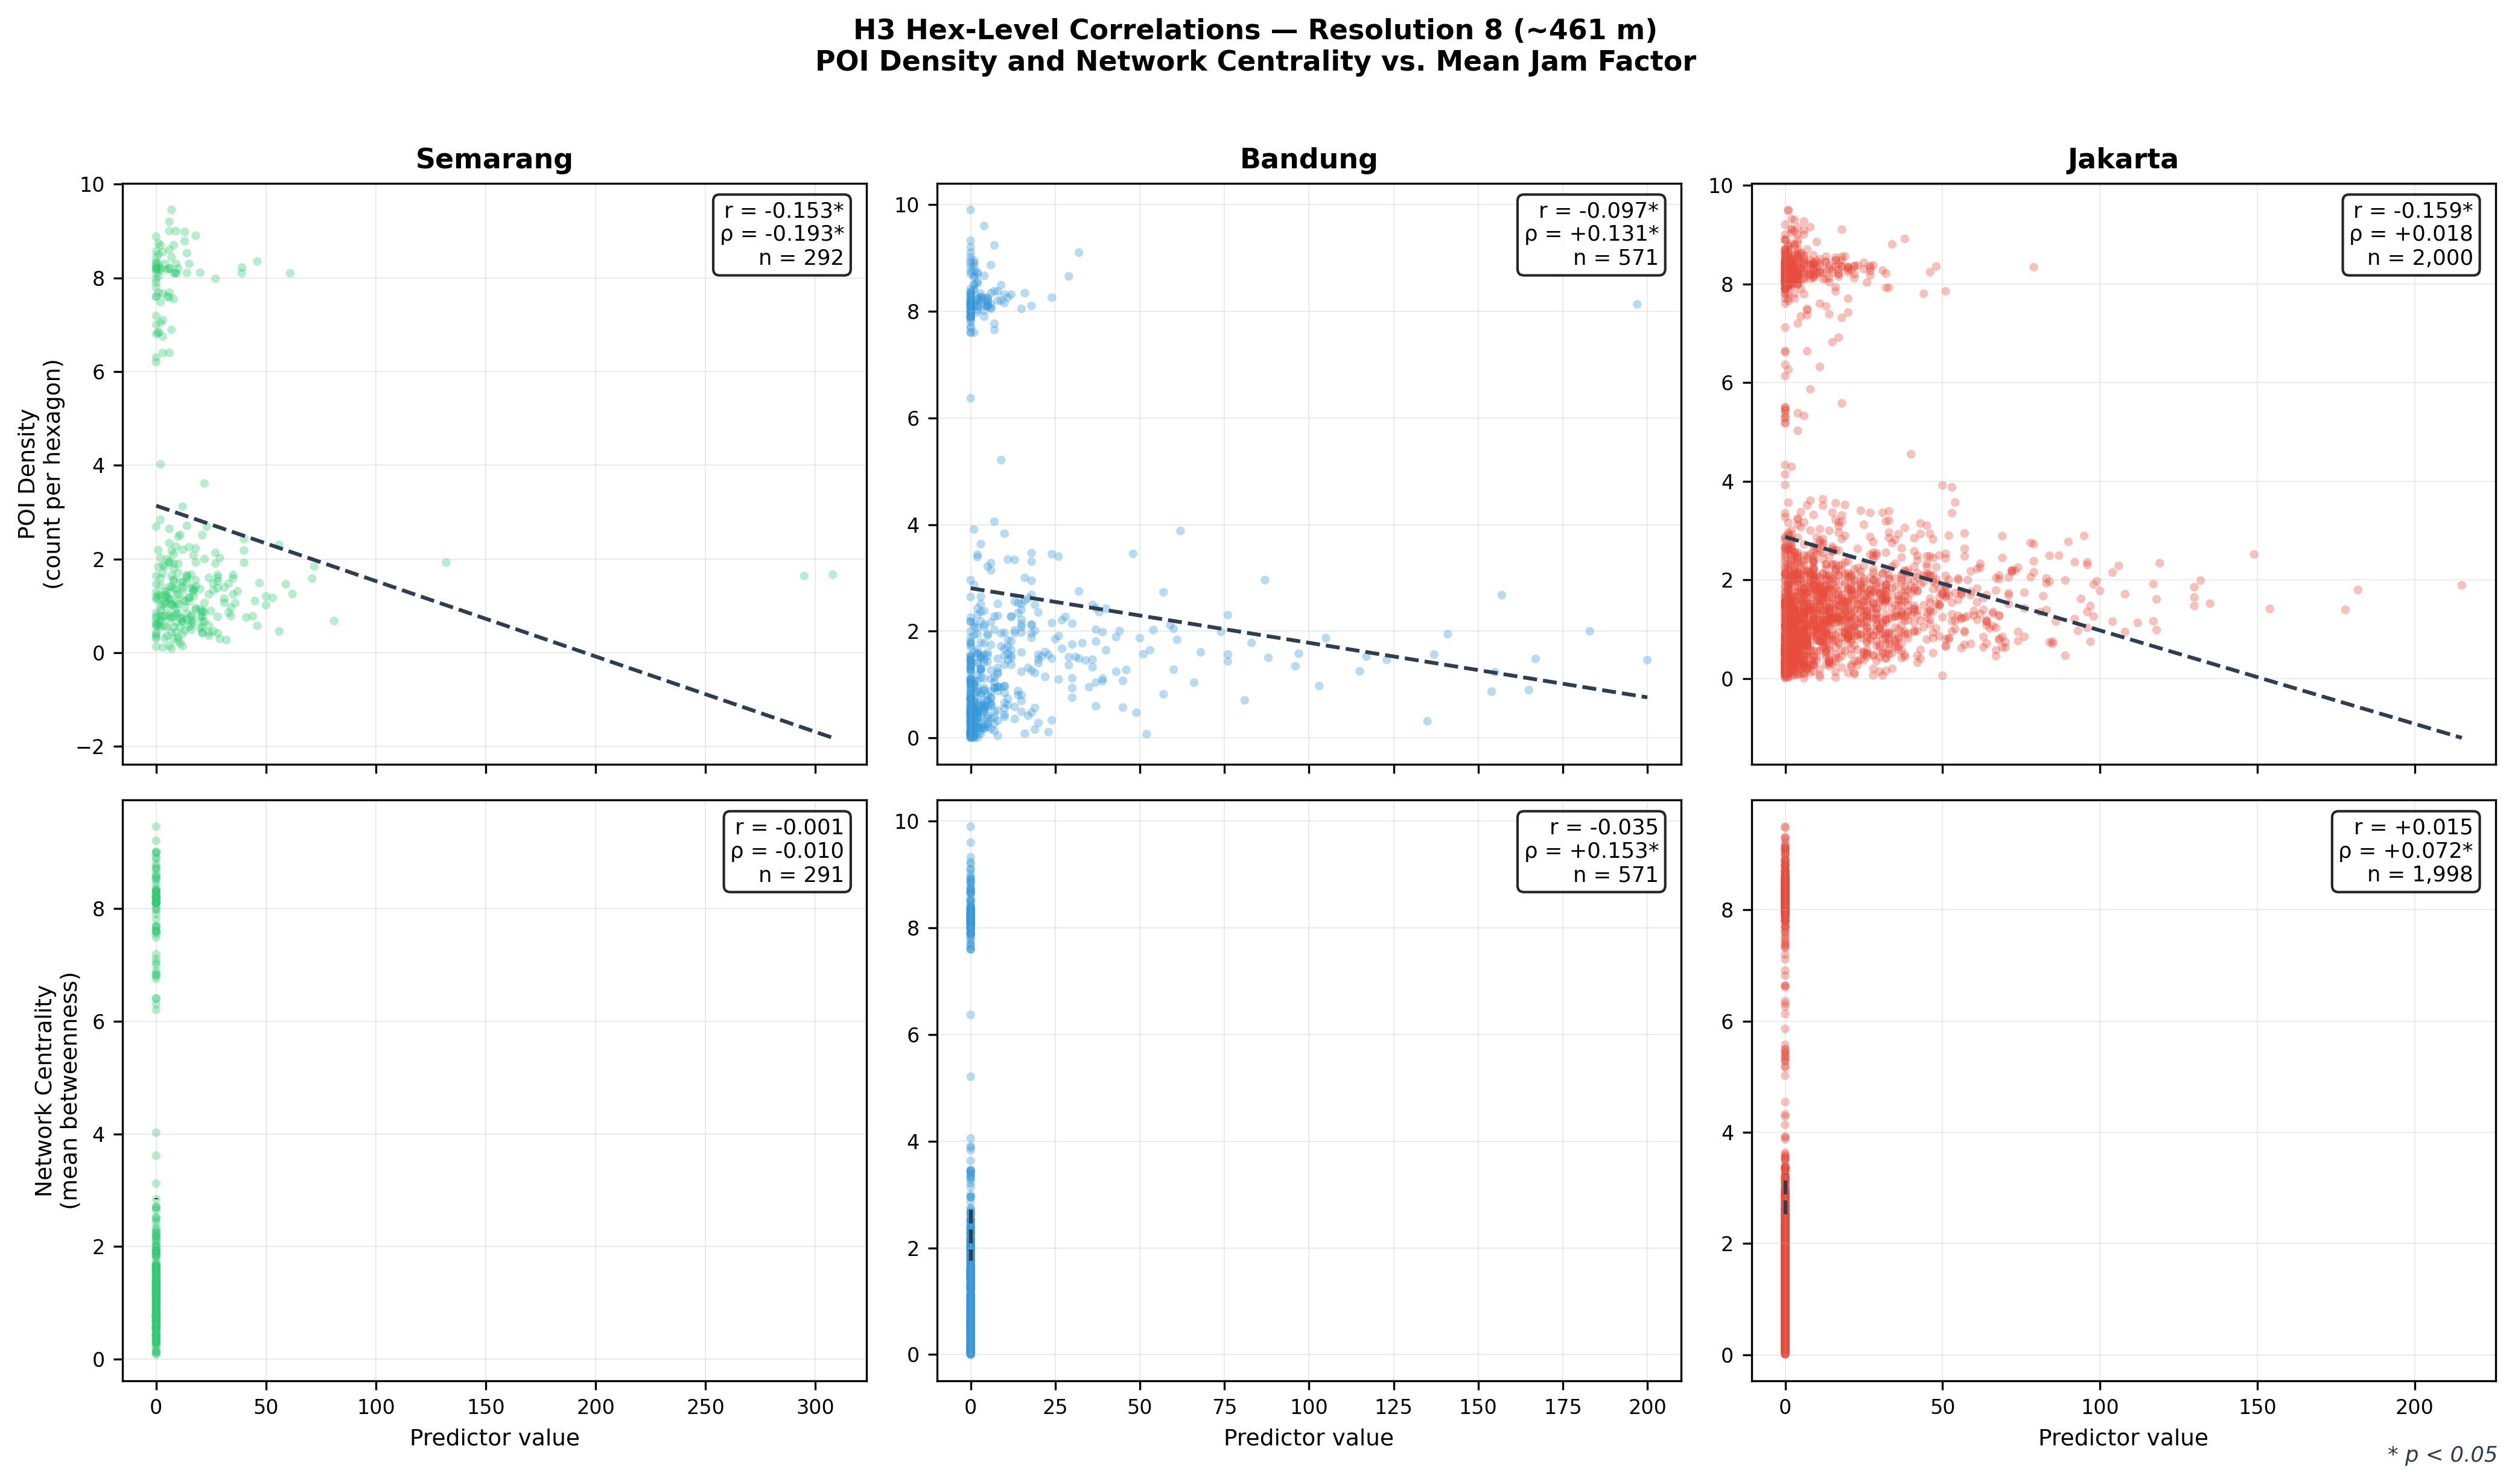
\includegraphics[width=\textwidth]{../figures/h3_correlation_panels.png}
\caption{Scatter plots of POI density (top row) and network centrality (bottom row) versus hex-level mean jam factor at H3 resolution~8. Dashed lines show OLS regression fits. Pearson $r$ and Spearman $\rho$ are annotated per panel; no significant correlation is detected in any city for either predictor.}
\label{fig:h3_correlation_panels}
\end{figure}

\begin{figure}[htbp]
\centering
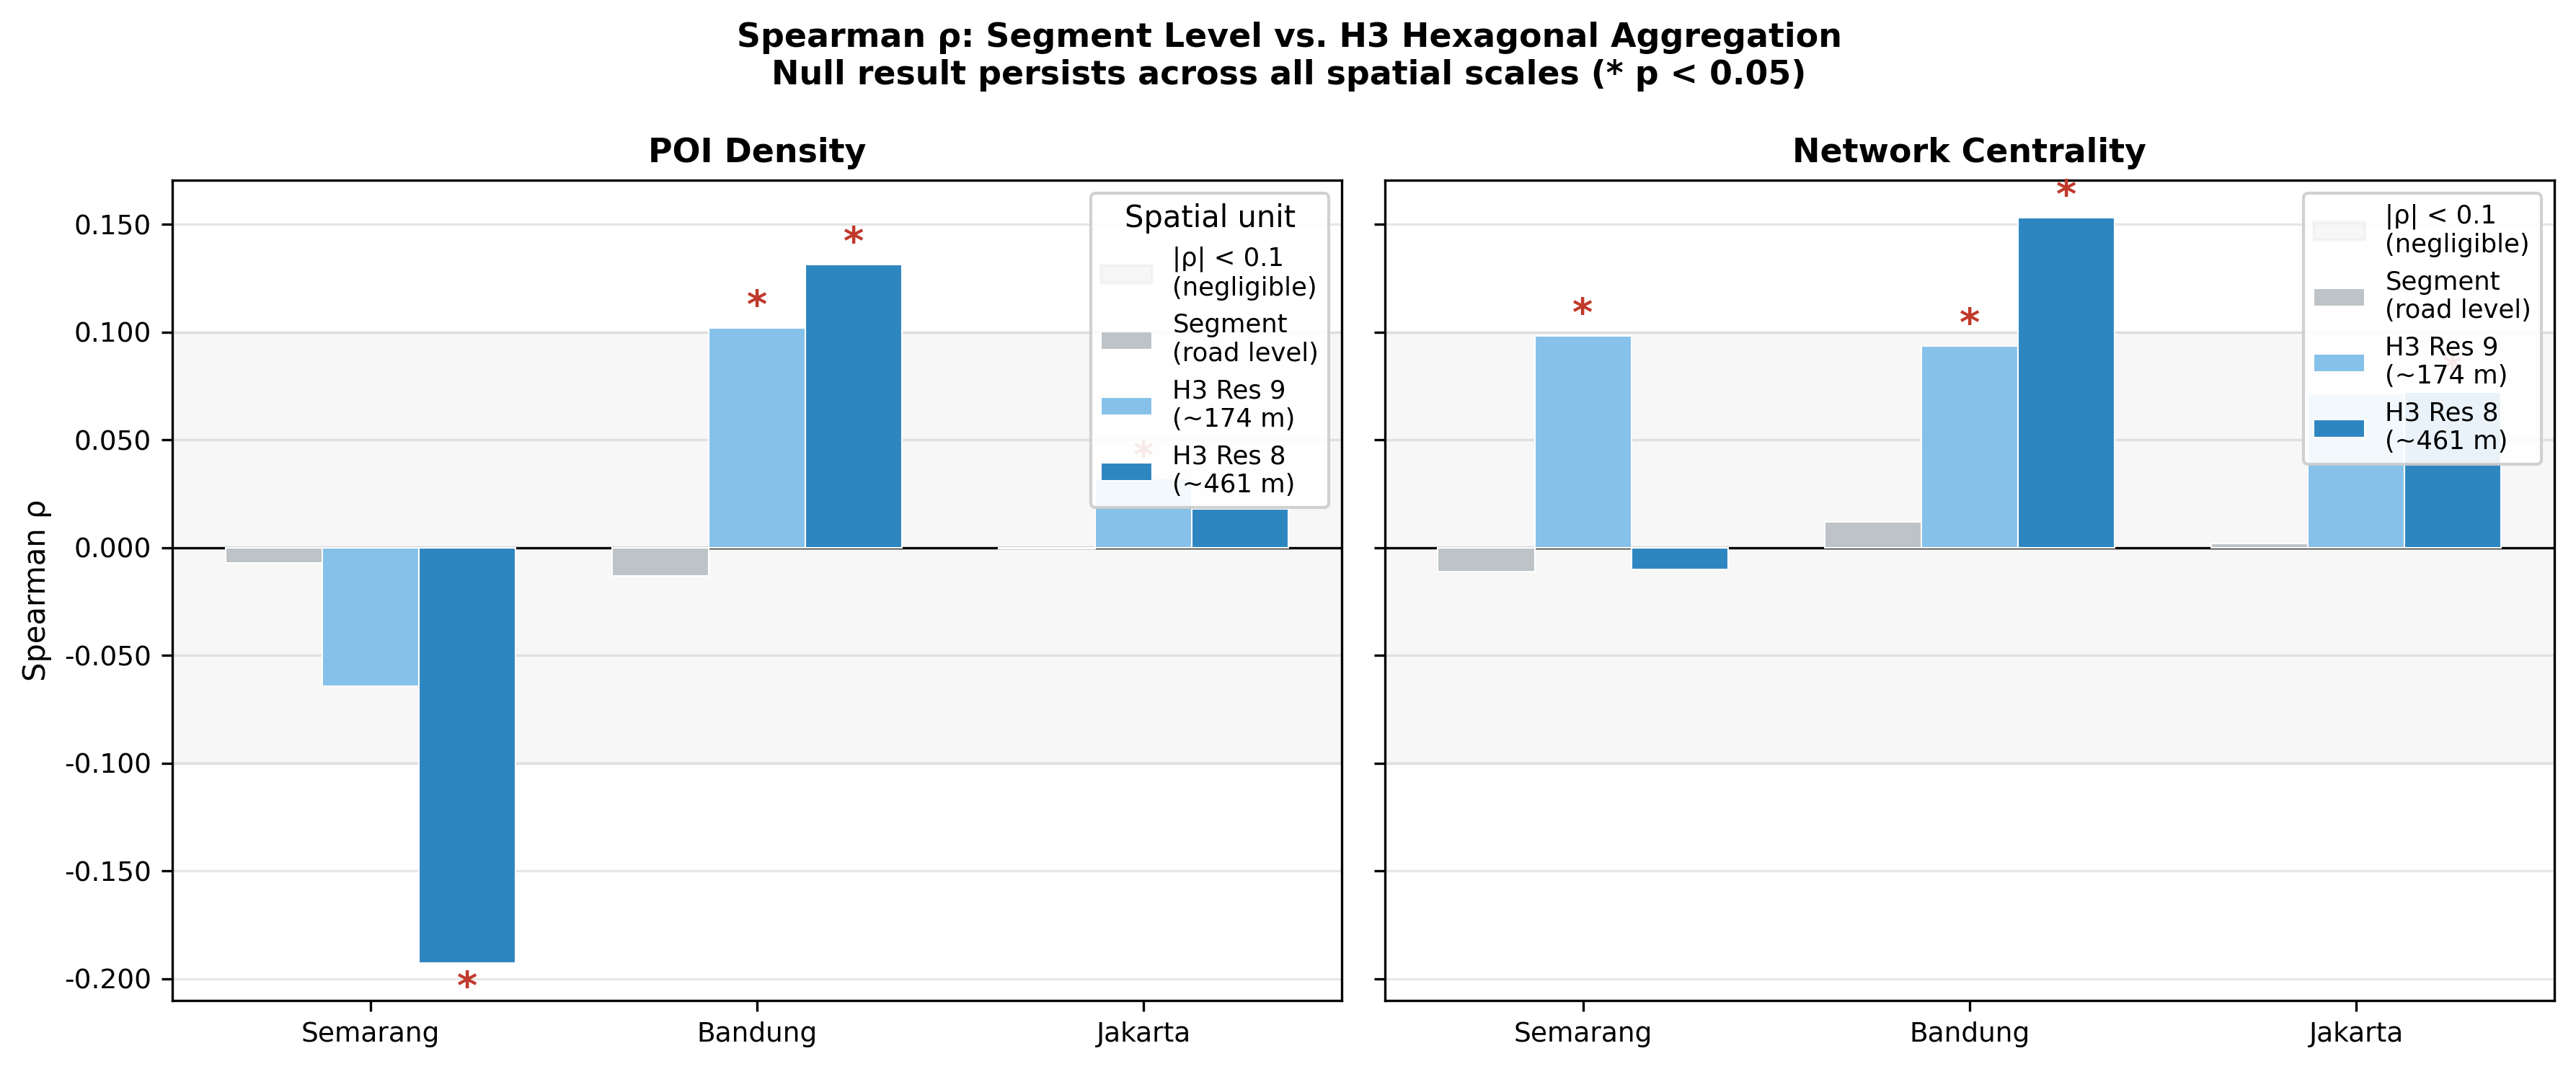
\includegraphics[width=0.85\textwidth]{../figures/h3_correlation_comparison.png}
\caption{Spearman $\rho$ for POI density (left) and network centrality (right) at three spatial scales: road segment, H3 resolution~9 ($\approx$174\,m), and H3 resolution~8 ($\approx$461\,m). The grey band marks the negligible-effect region ($|\rho|$ < 0.1). Correlations remain within the negligible band across all cities and scales, confirming that the null segment-level findings are not a modifiable areal unit artefact.}
\label{fig:h3_correlation_comparison}
\end{figure}

\subsection{Bottleneck and Capacity Drop Analysis}

\paragraph{Aggregate Capacity--Congestion Relationship}

Spatial join between HERE segments and filtered OSMnx networks achieved 95--98\% match rates. Contrary to the bottleneck hypothesis, \textbf{high-capacity roads show marginally higher congestion} than low-capacity roads in all cities (Table~\ref{tab:table13})---the opposite of capacity constraint predictions. All differences are non-significant (p > 0.05) with trivial effect sizes ($|d|$ < 0.08). This reversal reflects the HERE jam factor's normalization to free-flow speed: capacity effects are divided out by design. Pearson and Spearman correlations between capacity score and jam factor confirm near-zero relationships (Table~\ref{tab:table14}).

\begin{longtable}[]{@{}
  >{\raggedright\arraybackslash}p{(\linewidth - 14\tabcolsep) * \real{0.0606}}
  >{\raggedright\arraybackslash}p{(\linewidth - 14\tabcolsep) * \real{0.1718}}
  >{\raggedright\arraybackslash}p{(\linewidth - 14\tabcolsep) * \real{0.1918}}
  >{\raggedright\arraybackslash}p{(\linewidth - 14\tabcolsep) * \real{0.1918}}
  >{\raggedright\arraybackslash}p{(\linewidth - 14\tabcolsep) * \real{0.1918}}
  >{\raggedright\arraybackslash}p{(\linewidth - 14\tabcolsep) * \real{0.1920}}@{}}
\caption{Congestion comparison: Low- vs.\ high-capacity road segments}\label{tab:table13}\\
\toprule\noalign{}
City & Low-Capacity JF (SD) & High-Capacity JF (SD) & t & p-value & Cohen's d \\
\midrule\noalign{}
\endhead
\bottomrule\noalign{}
\endlastfoot
Jakarta & 1.36 (0.47) & 1.43 (0.47) & 1.87 & 0.062 & 0.08 \\
Bandung & 1.28 (0.49) & 1.34 (0.50) & 1.72 & 0.086 & 0.07 \\
Semarang & 1.15 (0.39) & 1.18 (0.41) & 1.01 & 0.312 & 0.06 \\
\end{longtable}

\begin{longtable}[]{@{}llllll@{}}
\caption{Capacity score--congestion correlations}\label{tab:table14}\\
\toprule\noalign{}
City & n matched & Pearson r & p-value & Spearman $\rho$ & p-value \\
\midrule\noalign{}
\endhead
\bottomrule\noalign{}
\endlastfoot
Jakarta & 14,539 & 0.025 & < 0.001 & 0.036 & < 0.001 \\
Bandung & 3,069 & 0.030 & 0.062 & 0.035 & 0.032 \\
Semarang & 1,076 & 0.037 & 0.192 & 0.040 & 0.154 \\
\end{longtable}

\paragraph{Capacity Drop Proximity Analysis}

Capacity drop locations were identified using the directed network graph method described in Section~\ref{sec:bottleneck}. Distance-to-nearest-drop shows no significant correlation with jam factor in any city (Table~\ref{tab:table15}), and t-tests comparing segments above versus below the median distance to nearest drop are non-significant (all p > 0.10). This indicates that proximity to capacity drops does not predict congestion levels.

\begin{longtable}[]{@{}llllll@{}}
\caption{Capacity drop proximity--congestion correlations}\label{tab:table15}\\
\toprule\noalign{}
City & n drops & Pearson r & p-value & Spearman $\rho$ & p-value \\
\midrule\noalign{}
\endhead
\bottomrule\noalign{}
\endlastfoot
Jakarta & 3,847 & 0.008 & 0.284 & 0.004 & 0.604 \\
Bandung & 1,102 & -0.010 & 0.604 & -0.014 & 0.435 \\
Semarang & 412 & -0.010 & 0.751 & -0.017 & 0.543 \\
\end{longtable}

\paragraph{Local Bottleneck Gradient Analysis}

Local bottleneck gradient analysis comparing segments with lower capacity than their K=10 network neighbors (local bottlenecks) against non-bottleneck segments yields null results across all cities (Table~\ref{tab:table16}). No significant differences emerge, with effect sizes below 0.05 in all cases. Combined with the preceding capacity drop and aggregate capacity results, four independent tests converge on the same conclusion: road capacity does not meaningfully predict congestion.

\begin{longtable}[]{@{}
  >{\raggedright\arraybackslash}p{(\linewidth - 14\tabcolsep) * \real{0.0606}}
  >{\raggedright\arraybackslash}p{(\linewidth - 14\tabcolsep) * \real{0.1718}}
  >{\raggedright\arraybackslash}p{(\linewidth - 14\tabcolsep) * \real{0.1918}}
  >{\raggedright\arraybackslash}p{(\linewidth - 14\tabcolsep) * \real{0.1918}}
  >{\raggedright\arraybackslash}p{(\linewidth - 14\tabcolsep) * \real{0.1918}}
  >{\raggedright\arraybackslash}p{(\linewidth - 14\tabcolsep) * \real{0.1920}}@{}}
\caption{Local bottleneck--congestion comparison}\label{tab:table16}\\
\toprule\noalign{}
City & Bottleneck JF (SD) & Non-Bottleneck JF (SD) & t & p-value & Cohen's d \\
\midrule\noalign{}
\endhead
\bottomrule\noalign{}
\endlastfoot
Jakarta & 1.43 (0.47) & 1.42 (0.47) & 0.35 & 0.724 & 0.02 \\
Bandung & 1.37 (0.51) & 1.35 (0.49) & 0.56 & 0.575 & 0.03 \\
Semarang & 1.20 (0.41) & 1.18 (0.40) & 0.61 & 0.543 & 0.04 \\
\end{longtable}

\begin{figure}
\centering
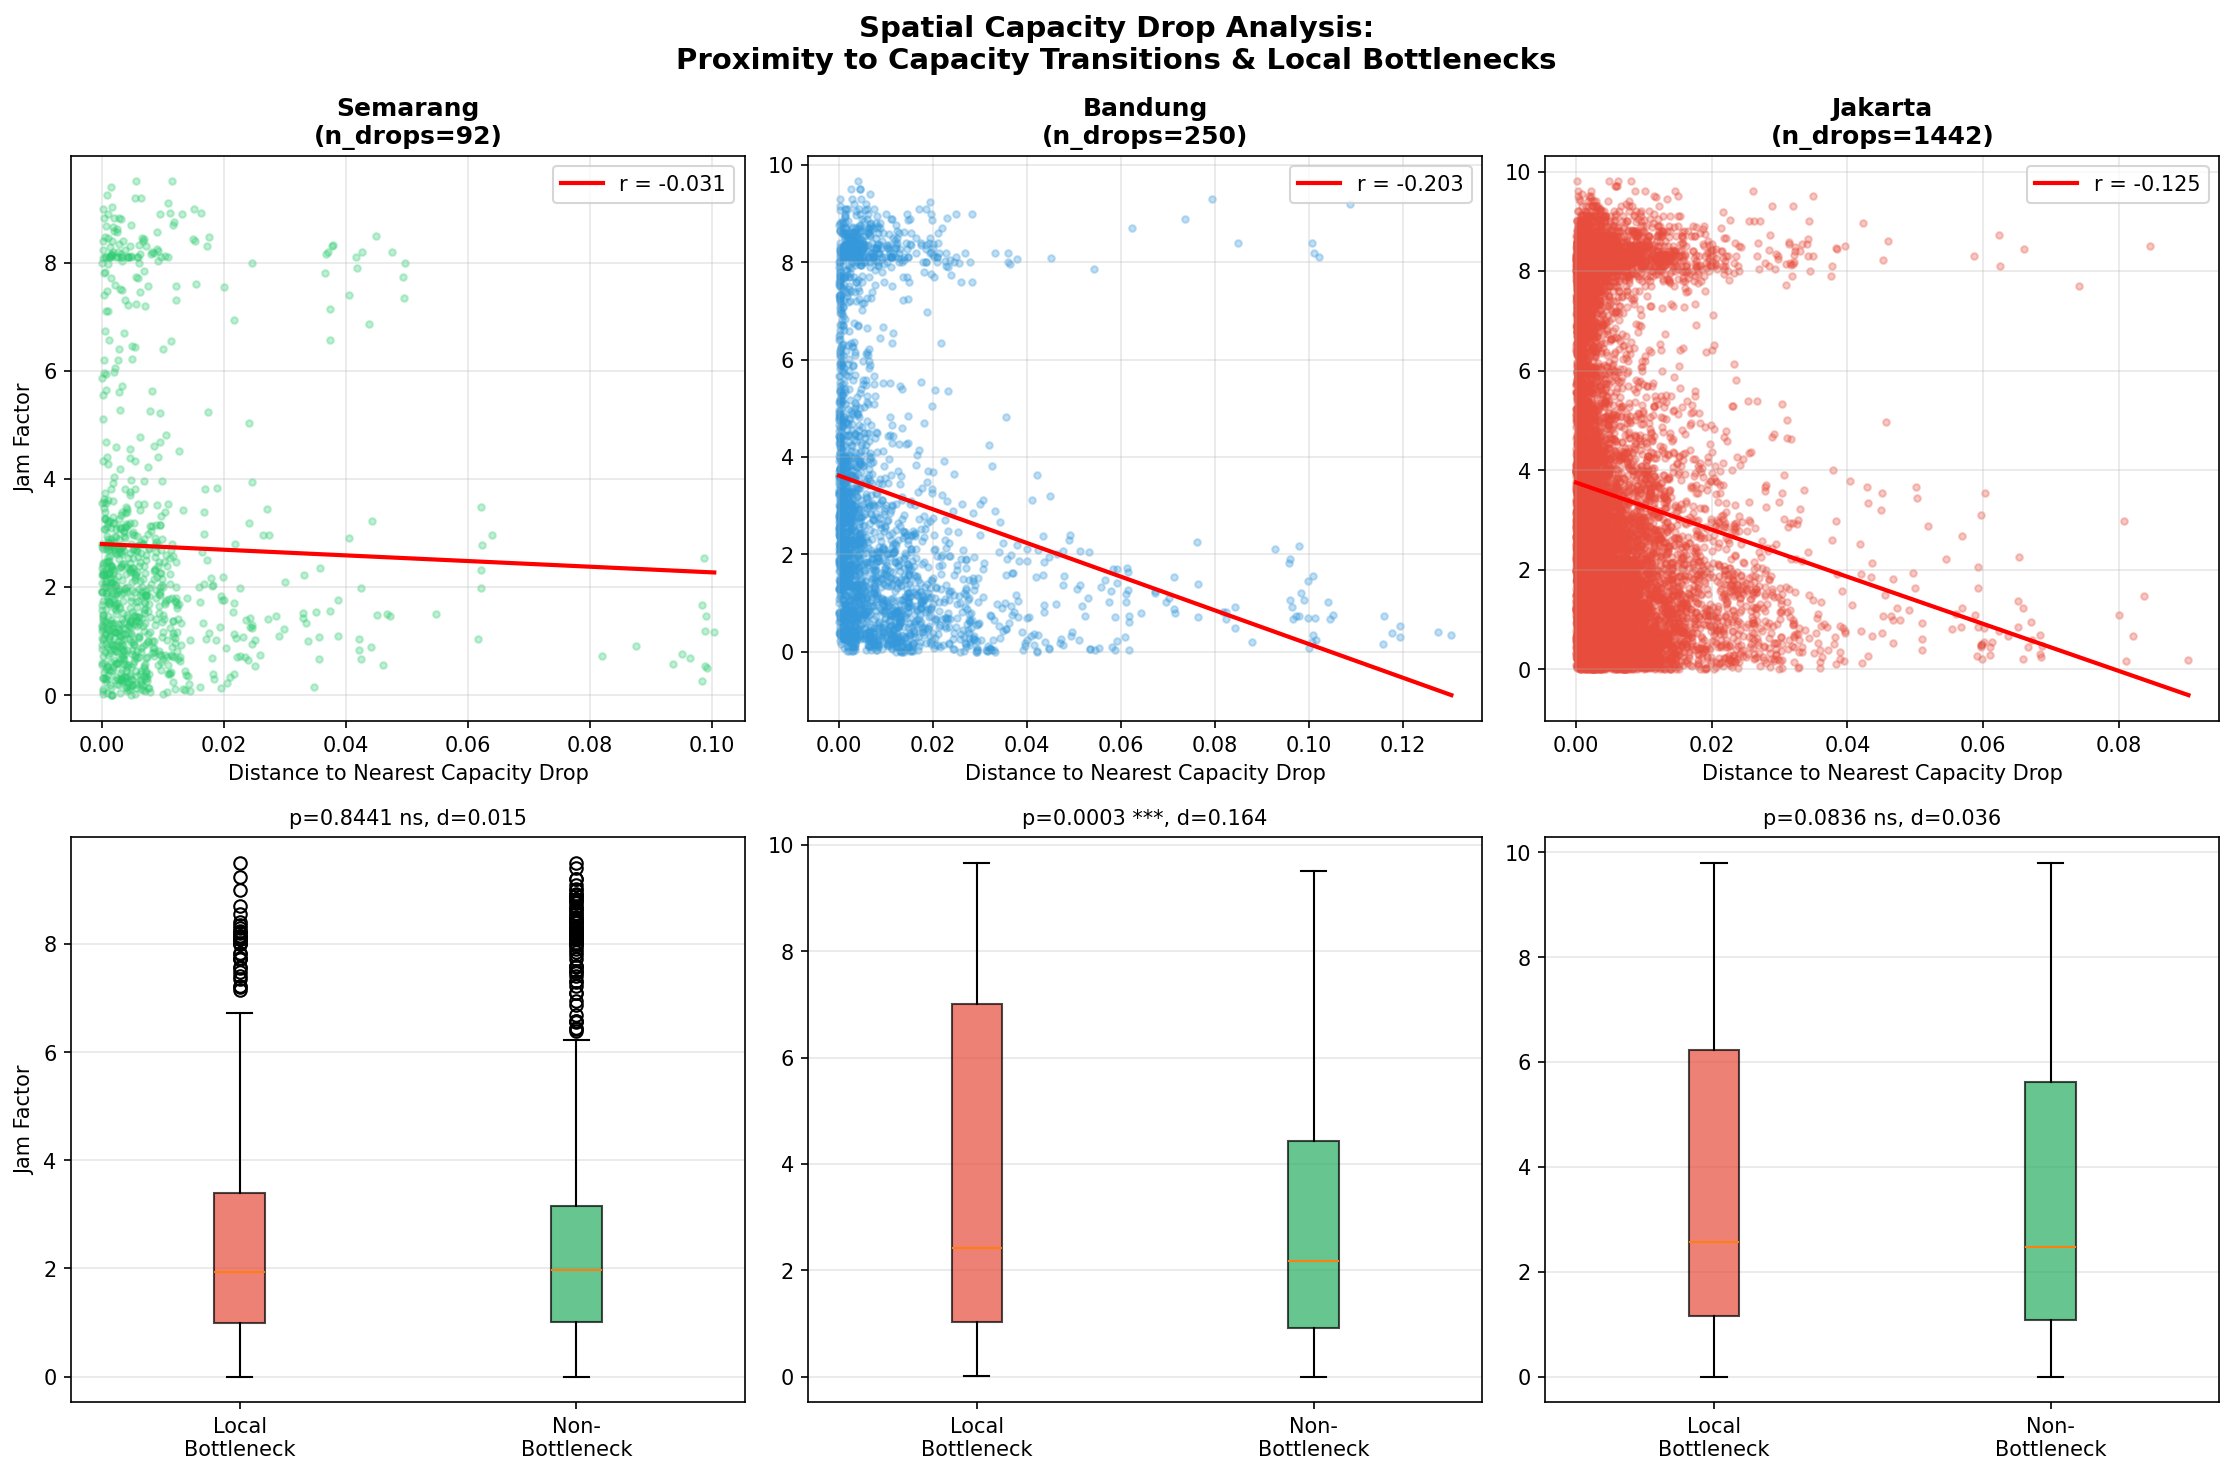
\includegraphics[width=\textwidth]{../figures/capacity_drop_spatial_analysis.png}
\caption{Spatial distribution of capacity drops and congestion - Jakarta}
\label{fig:capacity_drops}
\end{figure}

\subsection{Multilevel Variance Decomposition}

To rigorously partition temporal and spatial variance contributions---avoiding the methodological asymmetry of comparing $\eta^2$ from categorical ANOVA against $R^2$ from continuous predictors---we fit nested mixed-effects models using absolute speed (km/h) as the dependent variable (Table~\ref{tab:multilevel}).

The null model ICC indicates that 88--89\% of total speed variance lies between segments, reflecting fundamental differences in road design speeds (e.g., arterials vs.\ local roads). Within segments, time-of-day explains 57--67\% of speed fluctuations (pseudo-$R^2$ from the temporal model). Adding spatial predictors (betweenness centrality and free-flow speed) to the full model reduces between-segment variance by 74--79\% ($\Delta R^2$), but this reduction is almost entirely driven by free-flow speed---a proxy for road design capacity---rather than by network centrality. The betweenness coefficient is negative and significant ($p < 0.001$) in all cities, indicating that more central roads have slightly lower speeds after controlling for road type, consistent with higher traffic exposure on topologically important links.

\begin{longtable}[]{@{}lccccc@{}}
\caption{Multilevel model variance decomposition (absolute speed)}\label{tab:multilevel}\\
\toprule\noalign{}
City & Segments & ICC & Temporal $R^2$ & Spatial $\Delta R^2$ & $\beta_{\text{centrality}}$ \\
\midrule\noalign{}
\endhead
\bottomrule\noalign{}
\endlastfoot
Semarang & 1,056 & 89.4\% & 67.0\% & 79.1\% & $-$2,379*** \\
Bandung & 3,039 & 87.8\% & 63.1\% & 74.0\% & $-$5,632*** \\
Jakarta & 14,411 & 89.1\% & 56.5\% & 77.6\% & $-$27,605*** \\
\end{longtable}

\textit{Note: ICC = intraclass correlation from null model. Temporal $R^2$ = proportional reduction in within-segment variance. Spatial $\Delta R^2$ = proportional reduction in between-segment variance after adding centrality and free-flow speed. ***$p < 0.001$.}

The multilevel results provide a more nuanced picture than the previous $\eta^2$ vs.\ $R^2$ framing. Both temporal and spatial factors contribute meaningfully to speed variation, but they operate at different levels: temporal factors drive within-segment fluctuations (congestion dynamics), while spatial factors reflect between-segment differences (road infrastructure). Critically, the spatial variance explained by centrality \textit{alone} (without free-flow speed) is negligible ($\Delta R^2 < 1\%$ in all cities), confirming that network topology does not independently predict congestion after accounting for road type.

\begin{figure}[htbp]
\centering
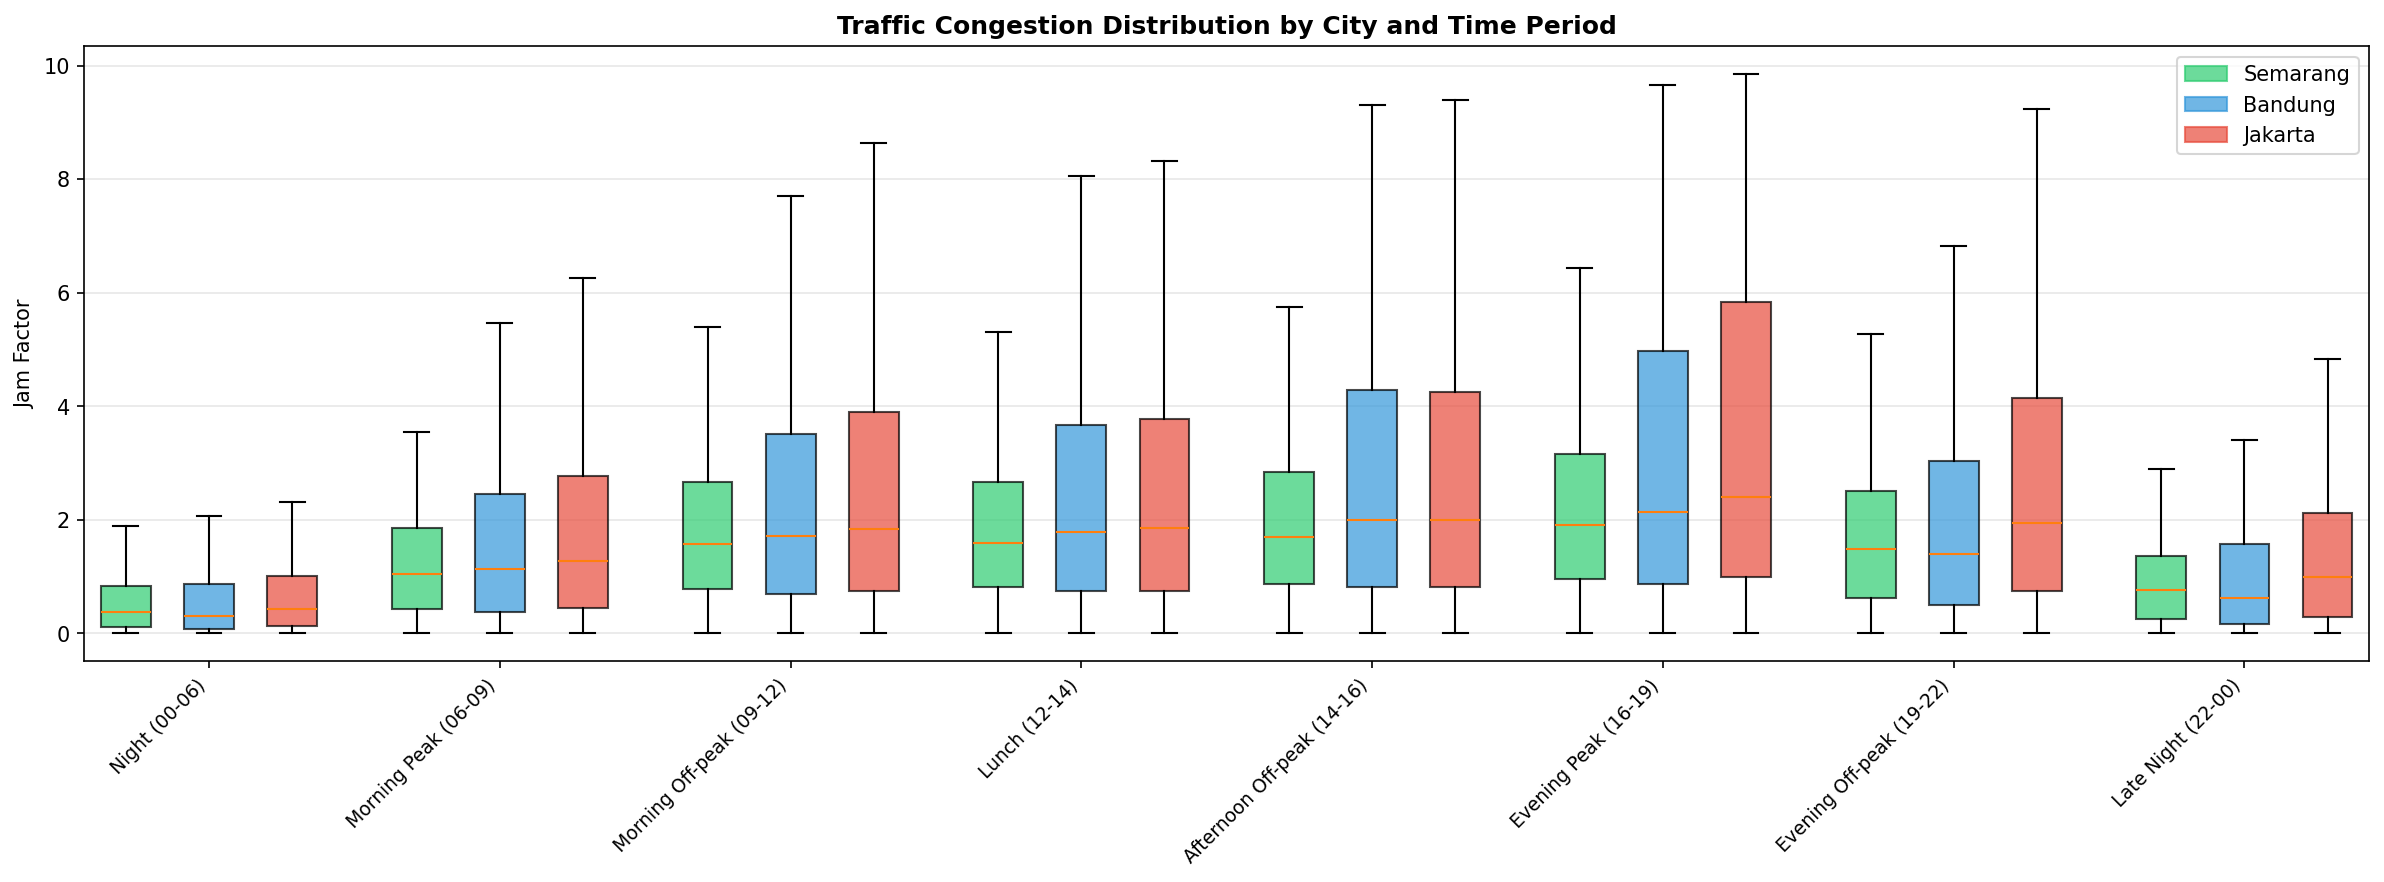
\includegraphics[width=\textwidth]{../figures/boxplot_comparison.png}
\caption{Jam factor distribution by temporal period and city}
\label{fig:boxplot}
\end{figure}

\section{Discussion}

The multilevel model reveals that urban congestion in three Indonesian cities operates fundamentally as a \textbf{demand synchronization problem}. Time-of-day explains 57--67\% of within-segment speed fluctuations---millions of commuters traveling simultaneously create congestion regardless of where they are in the network. This aligns with classical bottleneck theory: when demand exceeds capacity, queues form \citep{Vickrey1969,Arnott1993}, and the timing of demand matters more than the topology of supply. The consistency of this pattern across cities spanning a 20$\times$ population range---from Semarang (1.8M) to Jakarta metro (34M)---suggests demand synchronization is a scale-invariant congestion mechanism.

Four independent spatial tests (betweenness centrality, POI density, capacity score, and capacity drops) converge on the same conclusion: network topology and infrastructure characteristics do not independently predict congestion. The positive-control analysis strengthens this interpretation---the same analytical pipeline successfully detects spatial structure in road design speed ($R^2 = 0.60$--$0.71$) but not in congestion ($R^2 < 0.003$), ruling out methodological artefacts, insufficient power, or spatial matching errors. The H3 hexagonal aggregation (Section~\ref{sec:h3_robustness}) further confirms that null results persist at neighbourhood scales, addressing potential MAUP concerns.

The finding that high-capacity roads show marginally \textit{higher} congestion than low-capacity roads appears counterintuitive but reflects the HERE jam factor's normalization to free-flow speed. High-capacity roads (e.g., motorways) have higher free-flow speeds; when congestion occurs, the relative slowdown is proportionally larger even if absolute speeds remain higher than on lower-capacity roads. To test whether this normalization creates circular reasoning, we repeated all analyses using absolute speed (km/h) and speed reduction (free-flow minus current speed). The ANOVA results confirm temporal dominance across all metrics: $\eta^2$ = 8--10\% for jam factor and speed reduction, 5--6\% for absolute speed (Table~\ref{tab:speed_validation}). Similarly, network centrality correlations with absolute current speed are near zero ($R^2 < 0.003$; Table~\ref{tab:centrality_speed}), confirming that the null spatial finding is genuine rather than a normalization artifact. The moderate centrality--jam factor correlations ($R^2$ = 0.06--0.14) are mediated through free-flow speed: topologically important roads have higher design speeds, which amplifies normalized congestion scores without reflecting greater absolute congestion.

Our results align with emerging evidence that temporal patterns dominate spatial patterns in urban mobility. In a study of eight U.S. cities, time-of-day explained more variance in traffic than land-use or network topology \citep{Kang2020}. Similar temporal dominance was found in London \citep{Todd2019} and Beijing \citep{Zhang2017}. Our contribution extends this finding to Southeast Asian cities with unique traffic characteristics (high motorcycle shares) and demonstrates it using high-resolution, continuous monitoring data rather than survey or snapshot methods.

The practical implications are significant for Indonesian and comparable Southeast Asian cities. If congestion is primarily driven by demand synchronization, then conventional supply-side responses---road widening, interchange construction, capacity expansion---address a secondary factor while leaving the primary driver untouched. Our findings support prioritizing \textbf{demand management} interventions: congestion pricing to spread peak demand temporally (as implemented in Singapore, London, and Stockholm); flexible and staggered work schedules, which directly target the synchronization mechanism; and public transit expansion, which reduces per-capita road space consumption during peak hours. Indonesia's ongoing mass rapid transit investments in Jakarta (MRT, LRT) and bus rapid transit systems in Bandung and Semarang align with this logic. The consistency of the temporal dominance finding across cities spanning a 20$\times$ population range---from Semarang (1.8M) to Jakarta metro (34M)---suggests these policy implications are not scale-dependent and may generalize across the Indonesian urban hierarchy.

Several limitations warrant discussion. First, we analyze three cities in a single country; generalization to cities with different urban forms (e.g., grid-planned cities, cities with extensive rail networks) requires caution. Second, our spatial predictors do not include every possible factor (e.g., traffic signal density, public transit routes, population density, land-use mix). Jakarta's weak but significant neighbourhood-level spatial autocorrelation detected through H3 aggregation suggests that unmeasured spatial variables may play a role. Third, the 11-month period, while extensive, may not capture long-term infrastructure or land-use changes. Fourth, the multilevel model uses speed aggregated to eight time periods per segment; finer temporal resolution (e.g., hourly) might reveal additional within-segment dynamics not captured at the period level.

Future research should: (1) apply the pipeline to cities outside Indonesia to test generalizability across different urban forms and transport systems; (2) incorporate dynamic predictors (signal timing, transit schedules) alongside static network measures; and (3) investigate the drivers of Jakarta's neighbourhood-level spatial autocorrelation using population density and land-use data.

\section{Conclusion}

This study analyzed 264 million traffic observations across three Indonesian cities to empirically decompose congestion into temporal and spatial components. Our central finding is that congestion operates as a \textbf{demand synchronization phenomenon}: time-of-day explains 57--67\% of within-segment speed fluctuations, while network topology adds less than 1\% beyond road type. A positive-control test confirms that the same pipeline detects spatial structure in road design speed ($R^2 = 0.60$--$0.71$) but not in congestion ($R^2 < 0.003$), and cross-metric validation using absolute speed confirms these patterns are not normalization artefacts. Evening peak congestion exceeds daily averages by approximately 40\% across all three cities despite a 20$\times$ population range, consistent with a demand-driven mechanism. These findings support prioritizing demand management strategies---congestion pricing, flexible work schedules, public transit expansion---alongside infrastructure investment in rapidly urbanizing contexts.

The open-source pipeline developed for this study (\texttt{pip install traffic-congestion-pipeline}) enables reproducible, scalable traffic analysis and is readily extensible to other cities. We encourage researchers in developing countries---where traffic congestion poses the greatest challenges---to adopt and adapt these tools for their own contexts.

\section{Acknowledgements}

We acknowledge HERE Technologies for access to the Traffic API. The use of generative AI (Claude, Anthropic) for code development and statistical automation is disclosed per journal policy. All AI-generated outputs were reviewed and validated by the authors.

\section{CRediT Author Statement}

\textbf{Firman Hadi}: Conceptualization, Methodology, Software, Formal analysis, Data curation, Writing -- Original draft, Visualization.
\textbf{Yasser Wahyuddin}: Validation, Writing -- Review \& editing.
\textbf{L.M. Sabri}: Supervision, Writing -- Review \& editing.
\textbf{Agung Indrajit}: Supervision, Writing -- Review \& editing.

\section{Data Availability Statement}

The traffic flow data used in this study are available from HERE Technologies under an academic license. The Python pipeline, aggregated statistics, and analysis scripts are publicly available at: \url{https://github.com/firmanhadi21/traffic-analyses} (MIT License). Processed datasets are archived at Zenodo: \href{https://doi.org/10.5281/zenodo.18650759}{10.5281/zenodo.18650759}.

\bibliographystyle{elsarticle-harv}
\bibliography{references}

\end{document}
